% Specify the type of document
\documentclass[12pt]{article}

% Load a number of useful packages
\usepackage{graphicx}
\usepackage{amsmath,amssymb,amsfonts,amsthm}
 \usepackage[margin=1.0in]{geometry}
\usepackage[colorlinks=true]{hyperref}
\usepackage{cite}
\usepackage[caption=false,font=footnotesize]{subfig}


% Two more packages that make it easy to show MATLAB code
\usepackage[T1]{fontenc}
\usepackage[framed,numbered]{matlab-prettifier}
\lstset{
	style = Matlab-editor,
	basicstyle=\mlttfamily\small,
}

% Say where pictures (if any) will be placed
\graphicspath{{./pictures/}}

% Define title, author, and date
\title{AE353: Design Problem 02}
\author{Emilio Gordon}
\date{March 10, 2017}

% Start of document
\begin{document}

% Put the title, author, and date at top of first page
\maketitle


\section{Goal}
\lstinline!DesignProblem02! simulates a ``gravity-assisted under actuated robot arm'' that is similar to one proposed for wing-box assembly in aircraft manufacturing by Roy Assad. The robotic arm is equipped with two joints however, only one is motorized. The motor applies a torque about the first joint while the second joint is allowed to spin freely. Finally, the robotic arm is equipped with optical encoders to measure joint angles and joint velocities.
\\ \\
The goal is to make for the robot arm to reach a stable equilibrium and then for the tip of the robot arm to move in accordance to a sequence of reachable points in space given by a predefined function. This would simulate the behavior of a robotic arm working inside of an aircraft's wing creating rivets. A requirement for the model is established such that
\begin{itemize}
	%\item The system (first and second joint) must have a settling time of less than five seconds
	\item The second joint angle shall remain within  $\pm5^{\circ}$ of its instantaneous reference value throughout the duration of the simulation.
\end{itemize}
With this requirement in mind, a procedure for verification can be established. Verification ensures that the system meets the established requirements. Verification will be conducted through several methodologies and are as follows
\begin{itemize}
	\item The simulation will generate an error between the second angle and the instantaneous reference value.
	\item For every time interval, a steady-state error is computed
	\item Plot a steady-state error to time curve. On this curve, include a reference line to mark if and when your steady-state error has surpassed the value stated by the requirement.
	\item Analyze the plot. If values exceed  $\pm5^{\circ}$, the single requirement has been ignored and the simulation has failed.
\end{itemize}

\section{Model} \label{Model}
In order to achieve the task at hand, a linearized state-space model for the system must be created. The sensors on the joints of the robotic arm return information pertaining to the joint's angle and it's velocity. As a result, q is defined to be a matrix of joint angles while $\dot{q}$ is a matrix of joint velocities. Finally, the matrix $\tau$ represents the applied torques of the system.
\begin{equation}
\label{eqnset}
q = \begin{bmatrix} q_{1} \\ q_{2} \end{bmatrix}
\qquad
\dot{q} = \begin{bmatrix} v_{1} \\ v_{2} \end{bmatrix}
\qquad
\tau = \begin{bmatrix} \tau_{1} \\ 0 \end{bmatrix}
\end{equation}
It is seen in Equation Set \eqref{eqnset} that the matrix $q$ takes in the joint angles for both joints one and two. Is is also seen that the matrix $\dot{q}$ takes in the velocities at both joints one and two. Notice however, how $\tau$ has $\tau_{1}$ and zero. This is the consequence of the second joint not having a motor, therefore, being incapable of applying torque.
\\ \\
The motion of the robot is governed by ordinary differential equations with the form
\begin{equation}
\label{eqEOM}
M(q) \ddot{q} + C(q,\dot{q})\dot{q} + N(q,\dot{q}) = \tau,
\end{equation}
such that 
\begin{equation*}
M(q) \qquad C(q,\dot{q}) \qquad N(q,\dot{q})
\end{equation*}
are matrix-valued functions of $q$ and/or $\dot{q}$. These functions depend on a number of parameters include mass and moment of inertia.  Using the code provided in the DesignProblem02 document, the ordinary differential equations were retrieved. These equations of motion are complex and rigorous to compute. Through the use of Matlab, the equations of motion can be linearized entirely through programming. Figure \ref{figCodeEOM} demonstrates the code necessary to load the Equations of Motion for this system.
\\
\begin{figure}[h!]
\begin{lstlisting}
% Load the equations of motion.
load('DesignProblem02_EOMs.mat');
% Parse the equations of motion.
M = symEOM.M;
C = symEOM.C;
N = symEOM.N;
tau = symEOM.tau;
% Define symbolic variables that appear in the equations of motion.
syms q1 q2 v1 v2 tau1 real\end{lstlisting}
\caption{Code to retrieve a symbolic description of the equations of motion in MATLAB. \label{figCodeEOM}}
\end{figure}
\\
Having established the elements of the state-space model, the nonlinear system must be linearized in order to simplify calculations. An initial equilibrium matrix is utilized to demonstrate the states and input for which the system is at equilibrium. The initial equilibrium is chosen such that 
\begin{equation}
\label{equil}
x_{eqillibrium} = \begin{bmatrix}q_{1e}\\ q_{2e}\\ v_{1e}\\ v_{2e}\end{bmatrix} = \begin{bmatrix}0\\ 0\\ 0\\0\end{bmatrix} 
\end{equation}
This establishes that when the robotic arm has both joints at an angle of zero, their velocities will be zero and therefore stationary. The goal wishes to observe the behavior of the arm as it moves to reach a sequence of reachable points. As a result, by choosing an initial equilibrium of zero, controllability is predicted to be easier since gravity will be acting againt the motor rather than with.
\begin{figure}[h!]
\begin{lstlisting}
%Establish equations for qdot (velocity) and qdotdot (acceleration)
qd = [v1; v2];
qdd = inv(M)*(-C*qd-N+tau);
%Define an equilibrium point containing input equilibrium [state state state state input]
equil = [0 0 0 0 0];
%Linearization takes palce by taking the jacobian of the equations wrt. the equilibrium points
Alower = vpa(subs(jacobian(qdd,[q1 q2 v1 v2]),[q1 q2 v1 v2 tau1],equil));
A = [0 0 1 0; 0 0 0 1; Alower];
Blower = vpa(subs(jacobian(qdd,tau1),[q1 q2 v1 v2 tau1],equil));
B = [0; 0; Blower];
C = eye(size(A));
\end{lstlisting}
\caption{Code used to linearize the state-space system about equilibrium\label{figLinear}}
\end{figure}
The code in Figure \ref{figLinear} shows how easy computing the Jacobian and Linearizing the system can be. The results to the code in Figure \ref{figLinear}  is shown in Equation Set \eqref{eqnJacob} producing the A, B and C matrix for the state-space model.
\begin{equation}
\begin{aligned}
\label{eqnJacob} 
A {\left(\begin{bmatrix} {qdd}_{e} \end{bmatrix}, x_{eqil}\right)} = & \begin{bmatrix} 0 &  0 &  1 & 0 \\ 0 & 0 & 0 & 1 \\ 4.967 & -54.77 & -3.284 & -0.6294\\ -2.182 &  -10.50 &  -0.6294 & -0.3085\end{bmatrix}
\\ \\
B {\left(\begin{bmatrix} {qdd}_{e} \end{bmatrix}, x_{eqil}\right)} = 
\begin{bmatrix} 0 \\ 0 \\ 3.284 \\0.6294\end{bmatrix}
& \qquad
C {\left(\begin{bmatrix} {qdd}_{e}\end{bmatrix}, x_{eqil}\right)} =
\begin{bmatrix} 1 & 0 & 0 & 0\\ 0 & 1 & 0 & 0 \\ 0 & 0 & 1 & 0 \\ 0 & 0 & 0 & 1 \end{bmatrix}
& 
D {\left(\begin{bmatrix} {qdd}_{e}\end{bmatrix}, x_{eqil}\right)} = 
\begin{bmatrix} 0\end{bmatrix}
\end{aligned}
\end{equation}
\\ \\
The resulting state-space model is
\begin{align*}
\dot{x} &= Ax+Bu \\
y &= Cx
\end{align*}
such that the behavior of this linear system and of the original, nonlinear system will be approximately the same so long as $x$ and $u$ are close to equilibrium.
\section{Controller}
The controller implemented for this design problem is a closed-loop linear system implementing reference tracking which allows the robotic arm to track a desired reference point and remain asymptotically stable so long as that reference point is within the bounds of the physical arm. There are multiple types of controllers, each advancing upon the last.
\subsection{Open Loop Linear System}
The first controller implemented is one with a zero-input solution. This refers to the systems behavior without any torque being applied to it through joint one. This is useful for understanding the effects the controller will have on the system once an input has been implemented. The system when controlled by a zero-input solution is shown in Figure \ref{zeroInputSet}. Represented in Figure \ref{zeroInputSet.a} is the system initially at a position that equal to its' physical equilibrium (recall that this is a gravity-assisted system) it will remain in that position. However, if this system were to start at a location with a slight offset from equilibrium, it will become unstable as demonstrated in Figure \ref{zeroInputSet.b}. It is important to note that this system can be in equilibrium at two angle positions to be defined as "natural equilibrium". The first where $\begin{bmatrix}q_{1} & q_{2}\end{bmatrix} = \begin{bmatrix}0 & 0\end{bmatrix}$ and the second where  $\begin{bmatrix}q_{1} & q_{2}\end{bmatrix} = \begin{bmatrix}\pi & -\pi \end{bmatrix}$. Note that the former was the same as the equilibrium set for this problem. Also note that Figure \ref{zeroInputSet.a} is positioned at $\begin{bmatrix} q_{1} & q_{2} \end{bmatrix} = \begin{bmatrix} \pi & -\pi \end{bmatrix}$
\begin{figure}[h!]
\centering
\subfloat[Velocities and joint angles at equilibrium (stable)]{
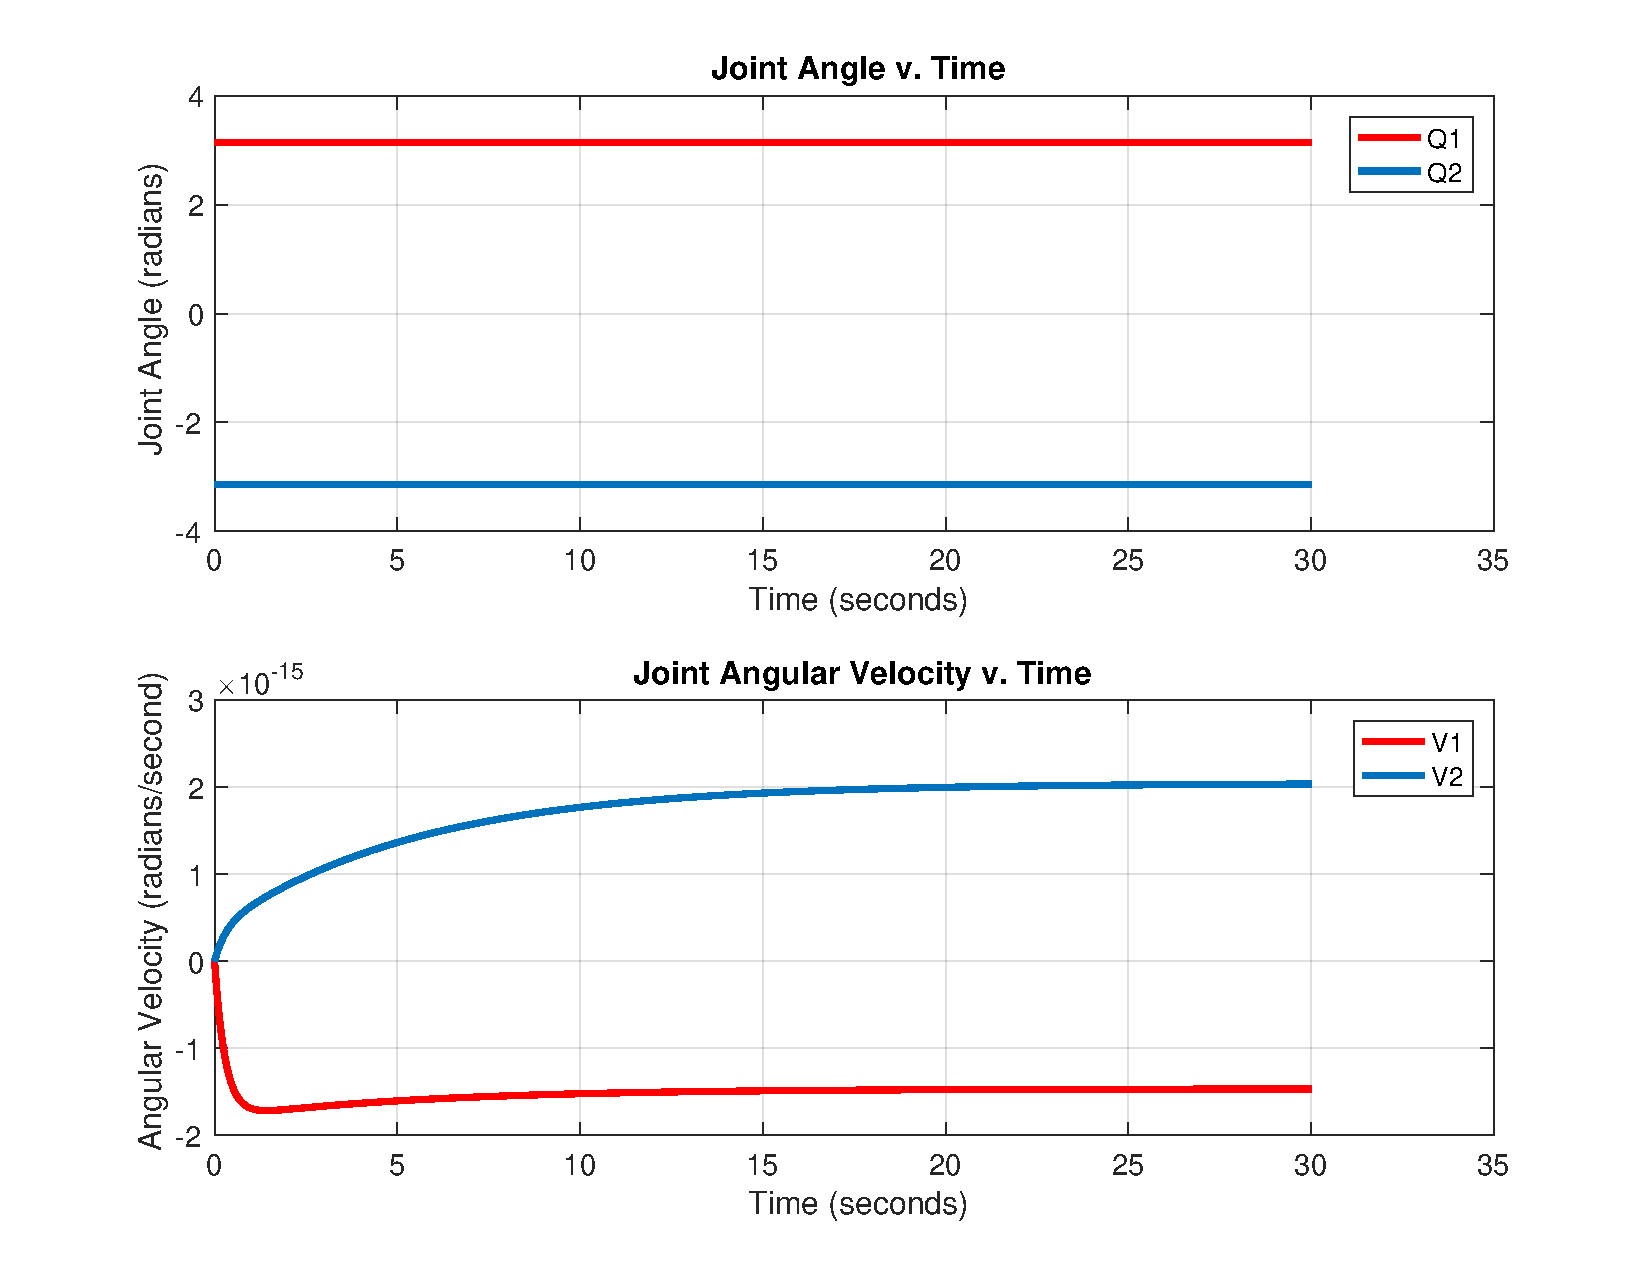
\includegraphics[width=.5\textwidth]{zisStable.pdf}
\label{zeroInputSet.a}}
\subfloat[Velocities and joint angles with a slight offset from equilibrium (unstable)]{
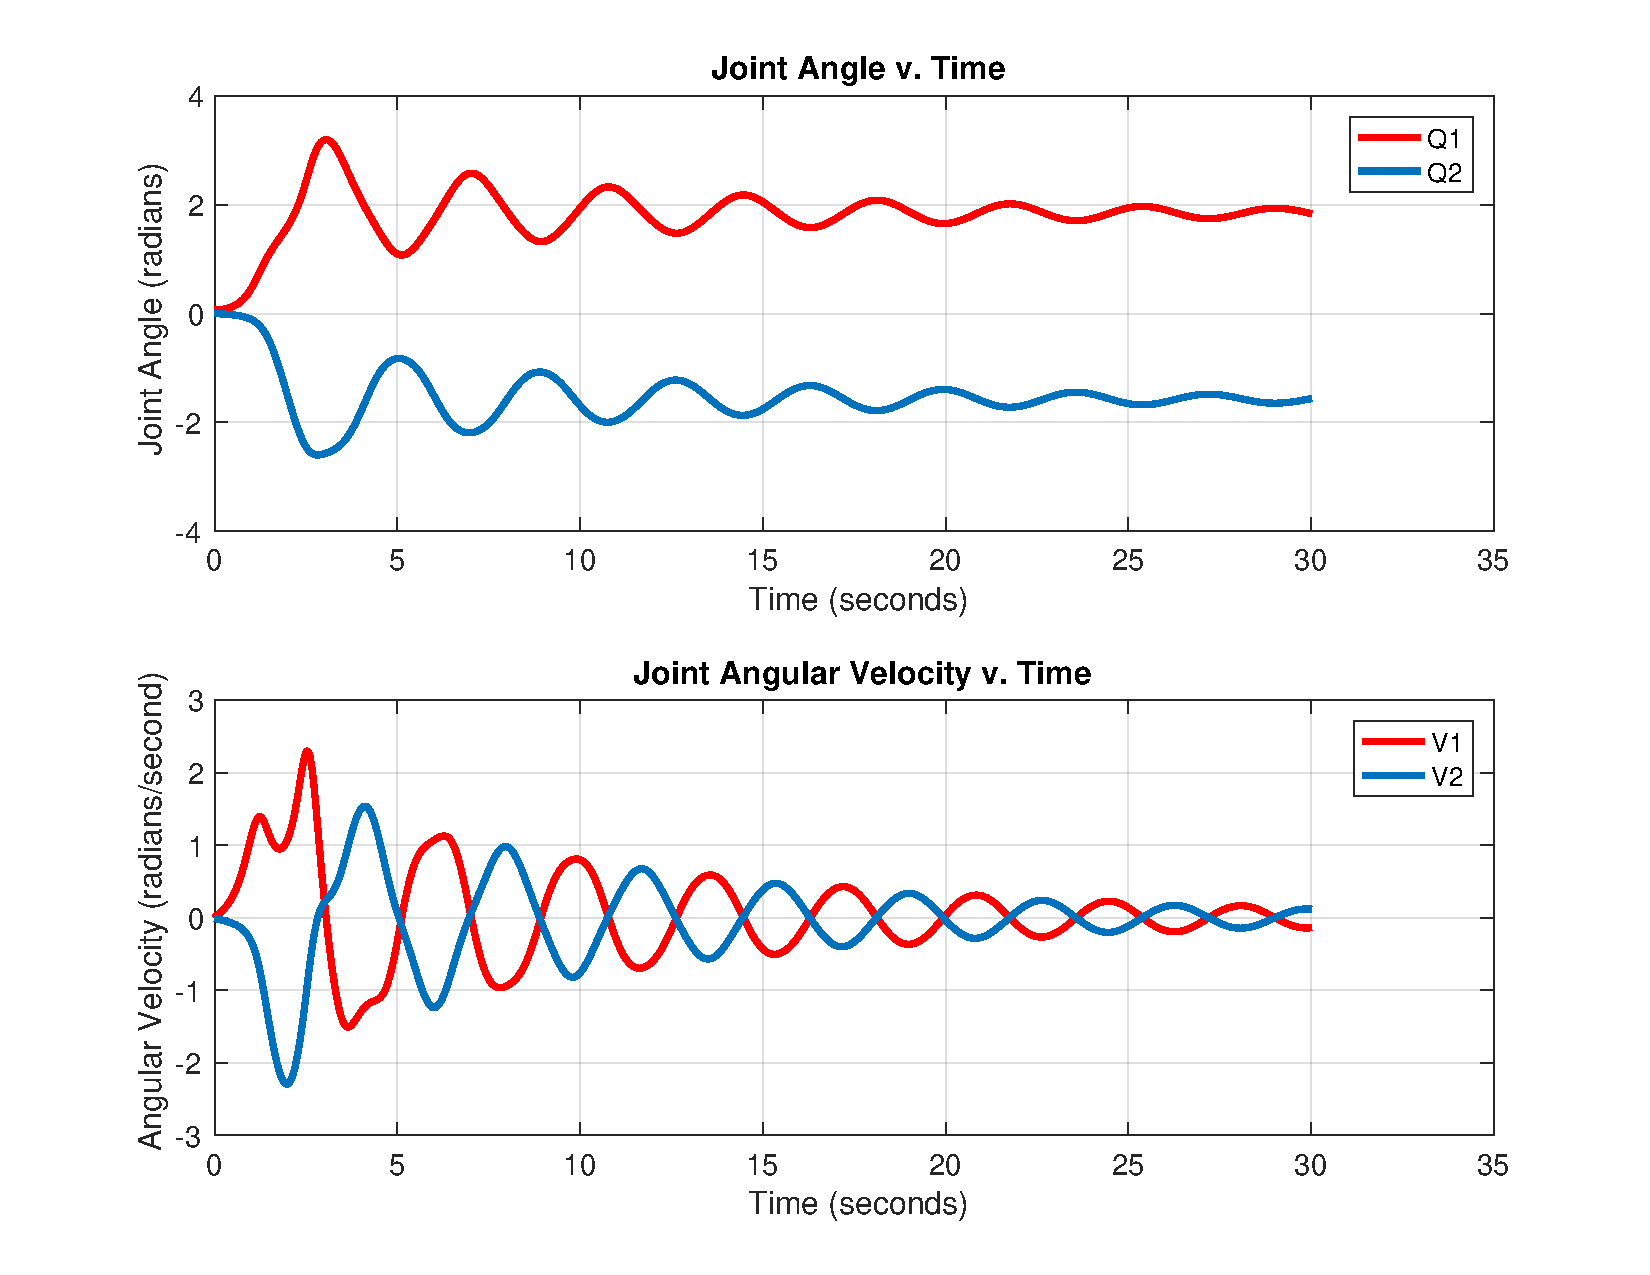
\includegraphics[width=.5\textwidth]{zisUnstable.pdf}
\label{zeroInputSet.b}}
\caption{Robotic arm during zero input solution}
\label{zeroInputSet}
\end{figure}
\subsubsection{Open Loop Controllability}
Not every system is controllable. If one wanted to make the entire state $x$ go to a desired value at some time, a controller must be implemented. By choosing some input $u(t)$, which is a function of time, the desired value should be reached. If it is possible for a system to move from state $x_{0}$ to any final state $x_{f}$ then the state-space system is considered controllable. Controllability is not always guaranteed so it is important to test for controllability before advancing with design. To solve this, the controllability matrix is implemented. The controllability matrix is associated with the original system so it is easy to compute. Figure \ref{controlmat} shows the calculation necessary to compute the controllability matrix.
\begin{figure}[h!]
\begin{lstlisting}
W = [B A*B A^2*B A^3*B]
\end{lstlisting} 
\vspace{5}
\begin{equation*} 
W = \begin{bmatrix}0 & 3.2840 & -11.1811 & 19.9813 \\ 
         0 & 0.6294 & -2.2613 & -6.0366 \\
    3.2840 & -11.1811 & 19.9813 & 6.4905 \\
    0.6294 & -2.2613 & -6.0366 & 37.4163
    \end{bmatrix}
\end{equation*}
\caption{Controllability matrix calculation and result.}
\label{controlmat}
\end{figure}
The system is controllable if and only if W, the controllability matrix, is full rank. This simply means that the matrix W is invertible. If the controllability matrix is invertible, it is possible to place eigenvalues at desired locations thereby giving the user control over the system. If the controllability matrix W is not invertible, then only some of the system's eigenvalues can be placed at desired locations, and the remaining eigenvalues cannot be moved. In the Figure \ref{rank} the rank between A and W are compared. Since they are the same, $rank(A)==rank(W)$, the open-loop linear system is controllable.
\begin{figure}[h!]
\label{rank}
\begin{lstlisting}
rank(A)
rank(W)
\end{lstlisting}
\caption{Controllability rank verification}
\end{figure}
\subsection{Closed Loop Linear System}
The second controller to be implemented is the state-feedback controller. State feedback is defined as a system in which the input depends on the state. State feedback has the input
\begin{align}
\label{eqn7}
u = -Kx
\end{align}
In equation \ref{eqn7}, $K$ represents a constant matrix whose values can be defined and manipulated to achieve equilibrium. The way in which state feedback,$u=-Kx$, differs from zero input response, $u=0$, is through the inputs ability to change. Previously, the system would act on its own wether it was stable or unstable due to gravity. However, with a state feedback, this is no longer the case. Torque is now applied to the robotic arm and with a proper formulation of $K$ the system can converge to the desired equilibrium points. 
\subsubsection{Linear Quadratic Regulator}
The $K$ matrix is found by implementing the Linear Quadratic Regulator (LQR), a state feedback controller that connects to the theory of optimal control. LQR is implemented easily through Matlab with the function 
\begin{lstlisting}[frame=single]
K = lqr(A,B,Q,R) %Linear Quadratic Regulator
\end{lstlisting}
The LQR function calculates the optimal gain matrix K such that:
\begin{itemize}
\item For a continuous-time state-space model, the state-feedback law $u = -Kx$  minimizes the cost function $J = \int (x'Qx + u'Ru) dt$ subject to the system dynamics  $dx/dt = Ax + Bu$
\item For a discrete-time state-space model, u[n] = -Kx[n] minimizes $J = \sum {x'Qx + u'Ru} $ subject to  $x[n+1] = Ax[n] + Bu[n]$.
\end{itemize}
The matrices $Q$ and $R$ are parameters that can be used to trade off error with effort. These matrices must be symmetric and be the right size. It is also important to note that
\begin{equation*}
Q \geq 0 \quad R > 0
\end{equation*}
As mentioned already, the matrices $Q$ and $R$ are parameters that can be used to trade off error with effort. This can be thought of as penalties with accordance to the states and inputs of the system. The more any of these are penalized, the less willing to change they will be. For example, if $v_{2}$, the angle velocity of joint two, had a high penalty, it would be more penalized and therefore, make smaller changes to avoid penalization. It is important to understand that $Q$ refers to penalties acting on the systems states and $R$ refers to penalties acting on the systems inputs. Equation \ref{QandR} establishes the $Q$ and $R$ matrix chosen to best achieve the goal.
\begin{equation}
Q = \begin{bmatrix}
100 & 0 & 0 & 0 \\ 0 & 10000 & 0 & 0 \\ 0 & 0 & 1 & 0 \\ 0 & 0 & 0 & 1
\end{bmatrix}
\qquad  
R = \begin{bmatrix}1\end{bmatrix}
\label{QandR}
\end{equation}
It is seen here that highly penalizing the angle of joint one $q_{1}$ and joint two $q_{2}$ resulted in the most optimal Q value. This will be explained further later in this section.
\\ \\
With the establishment of a $Q$ and $R$ matrix, the Matlab function lqr() resulted in a K which, when implemented into the state-feedback input of $u=-Kx$ allowed the system to reach equilibrium. Figure \ref{StateFeedbackSet1} show the system reaching an equilibrium from the initial position of $\begin{bmatrix} q_{1} & q_{2} \end{bmatrix} = \begin{bmatrix} \pi & -\pi \end{bmatrix}$. This is a complicated maneuver to accomplish since the robotic arm is battling gravity the entire way.  Alternatives to this are shown in Figure \ref{StateFeedback.c} and Figure \ref{StateFeedback.d} where the robotic arm has a random initial value. These initial conditions require much less work to be done and therefore converge faster. Regardless of the initial condition however, the arm converges to the equilibrium. 
\begin{figure}[h!]
\centering
\subfloat[Equillibirum via State Feedback]{
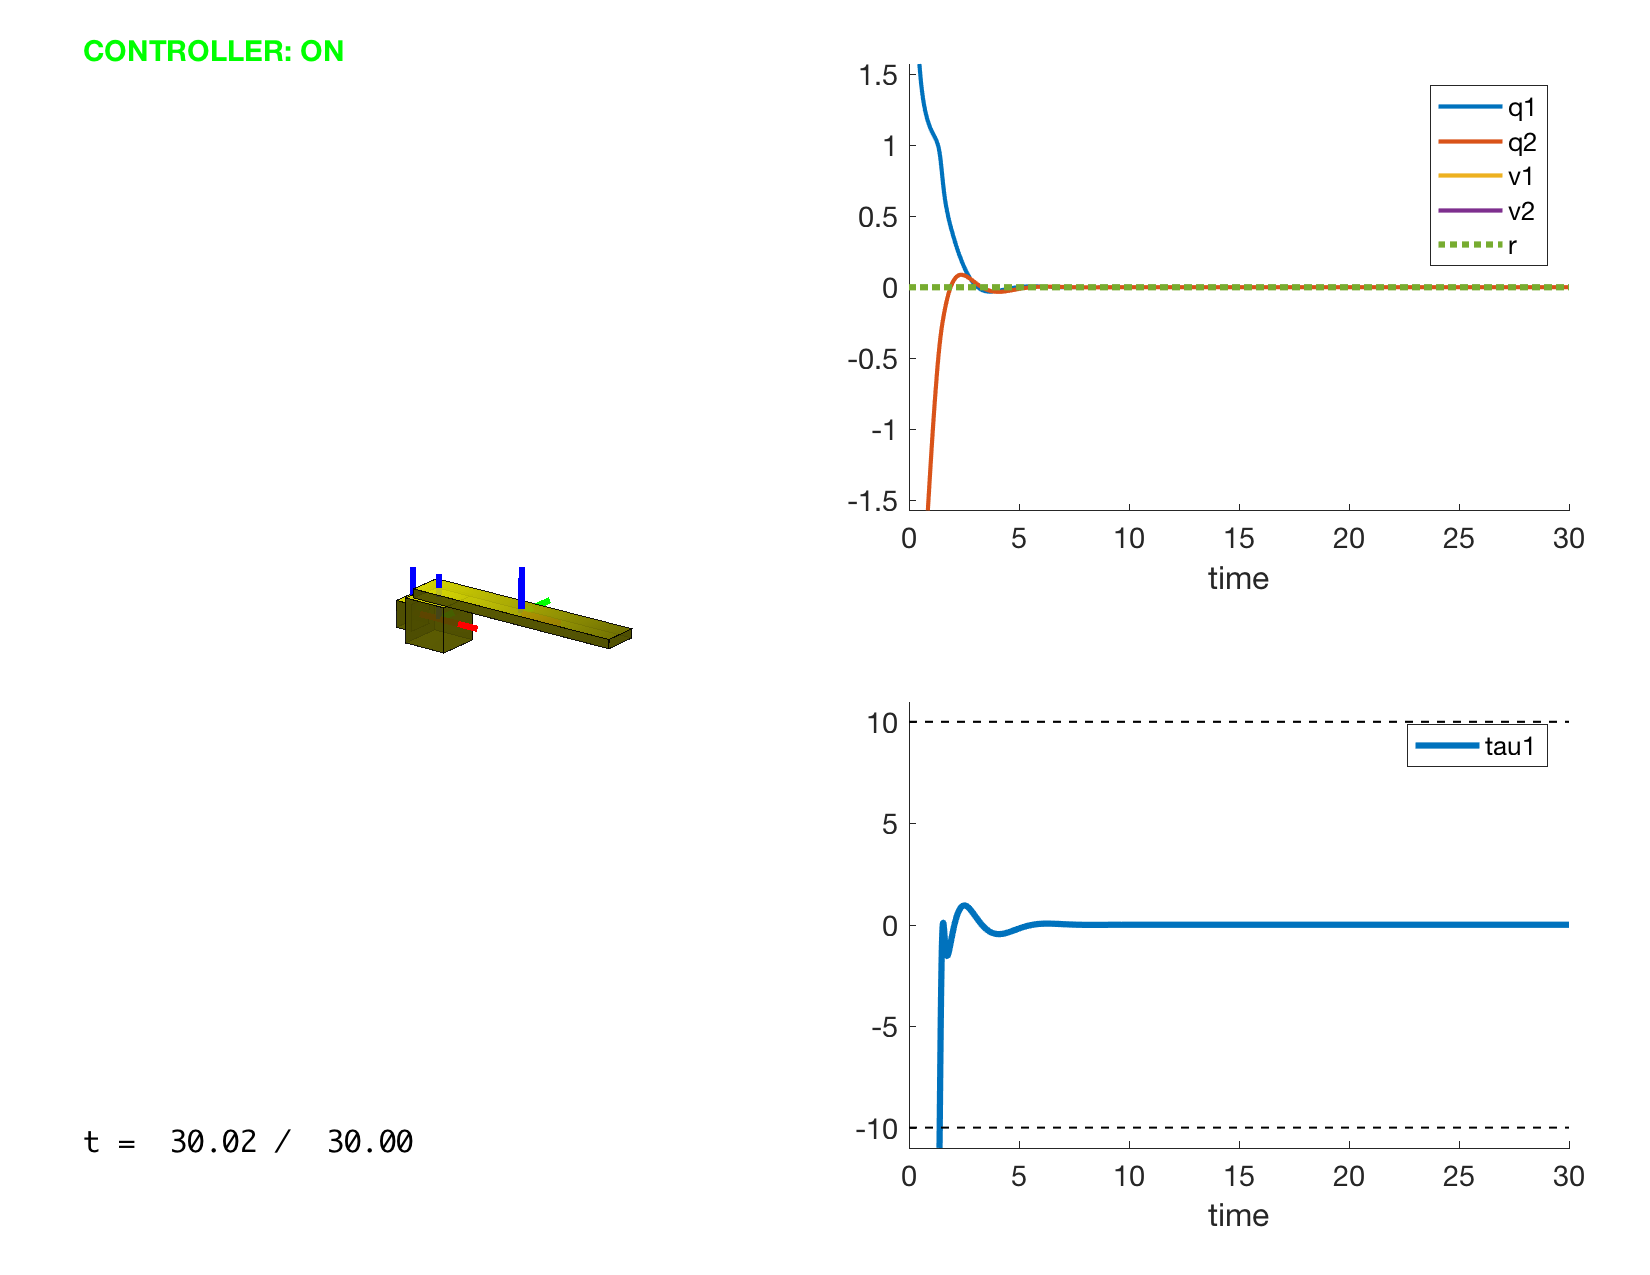
\includegraphics[width=0.5\textwidth]{pleasework.pdf}
\label{StateFeedback.a}}
\subfloat[Robotic arm with initial 
	\begin{equation*}\begin{bmatrix} q_{1} & q_{2}\end{bmatrix}=\begin{bmatrix}\pi & -\pi\end{bmatrix}\end{equation*}
]{
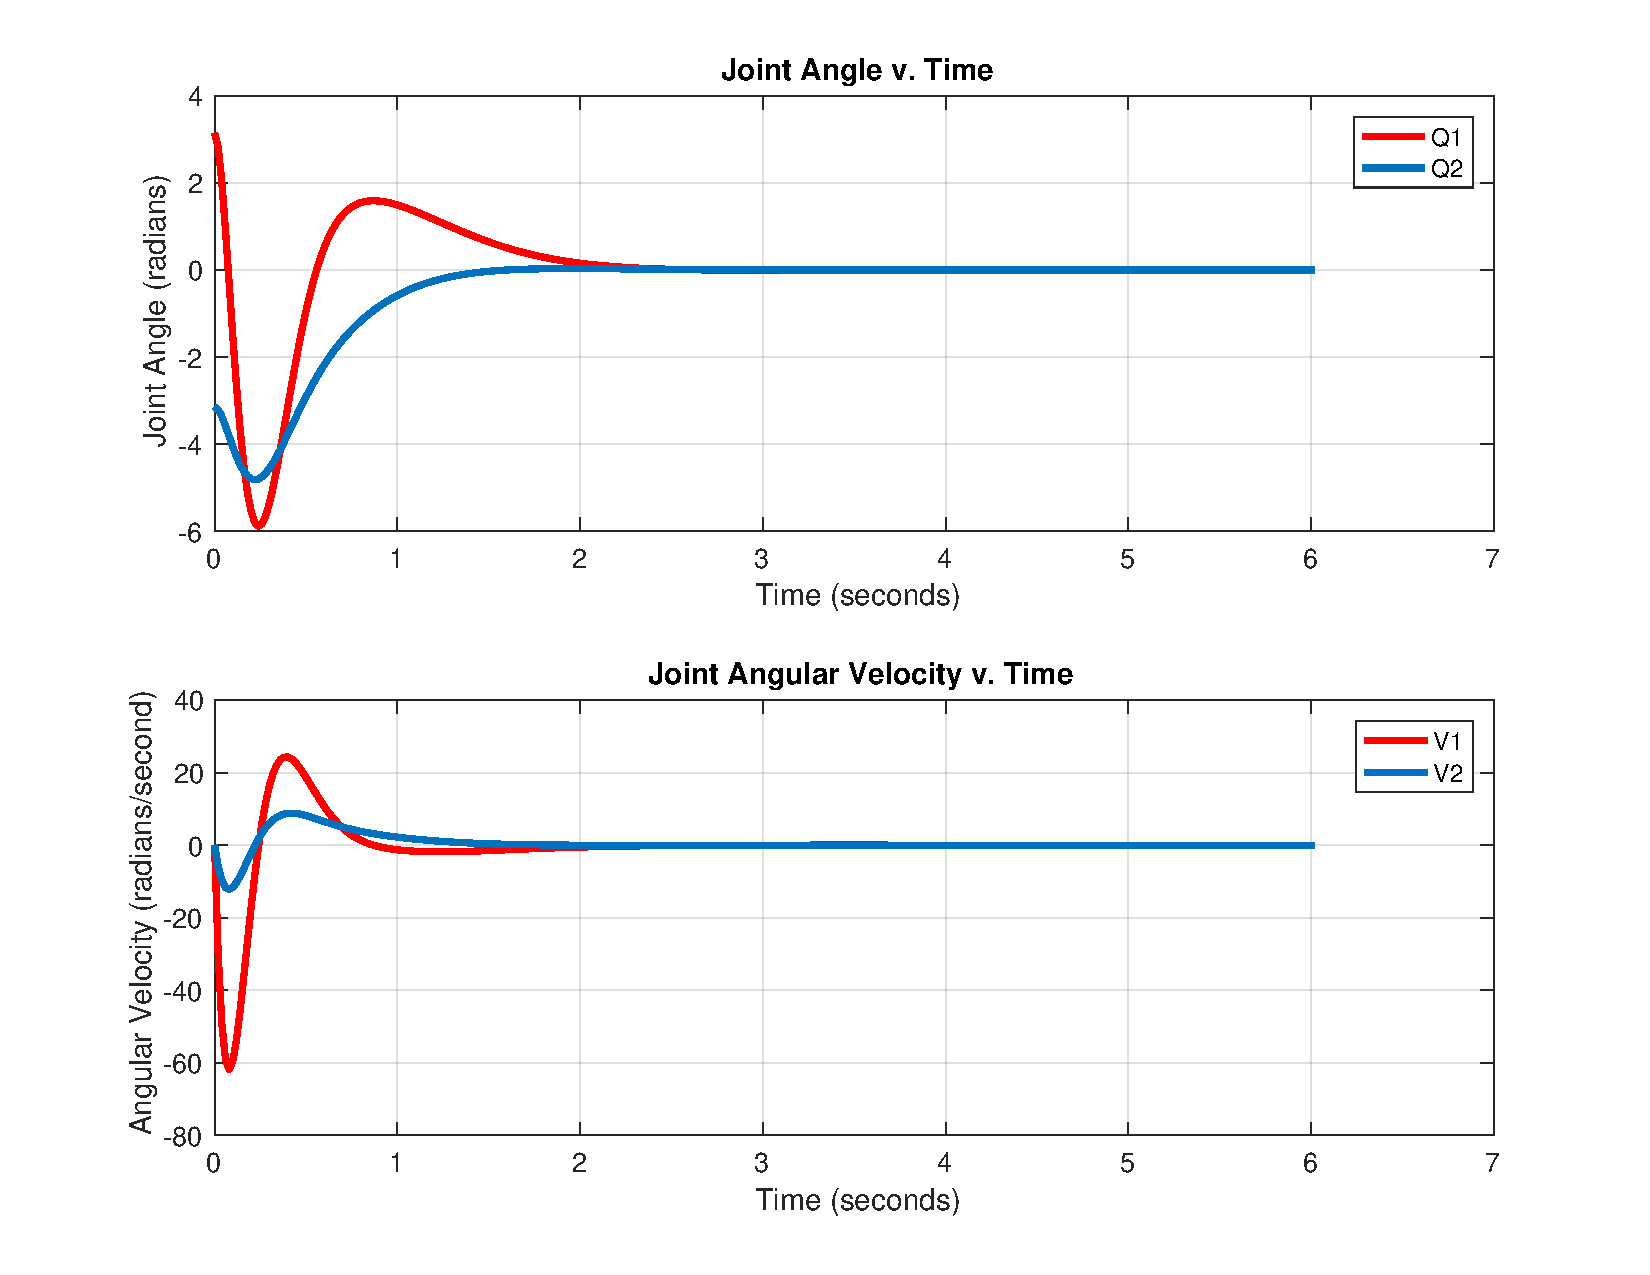
\includegraphics[width=0.5\textwidth]{SFfromPiPi.pdf}
\label{StateFeedback.b}}
 \\
\subfloat[Robotic arm with random initial conditions]{
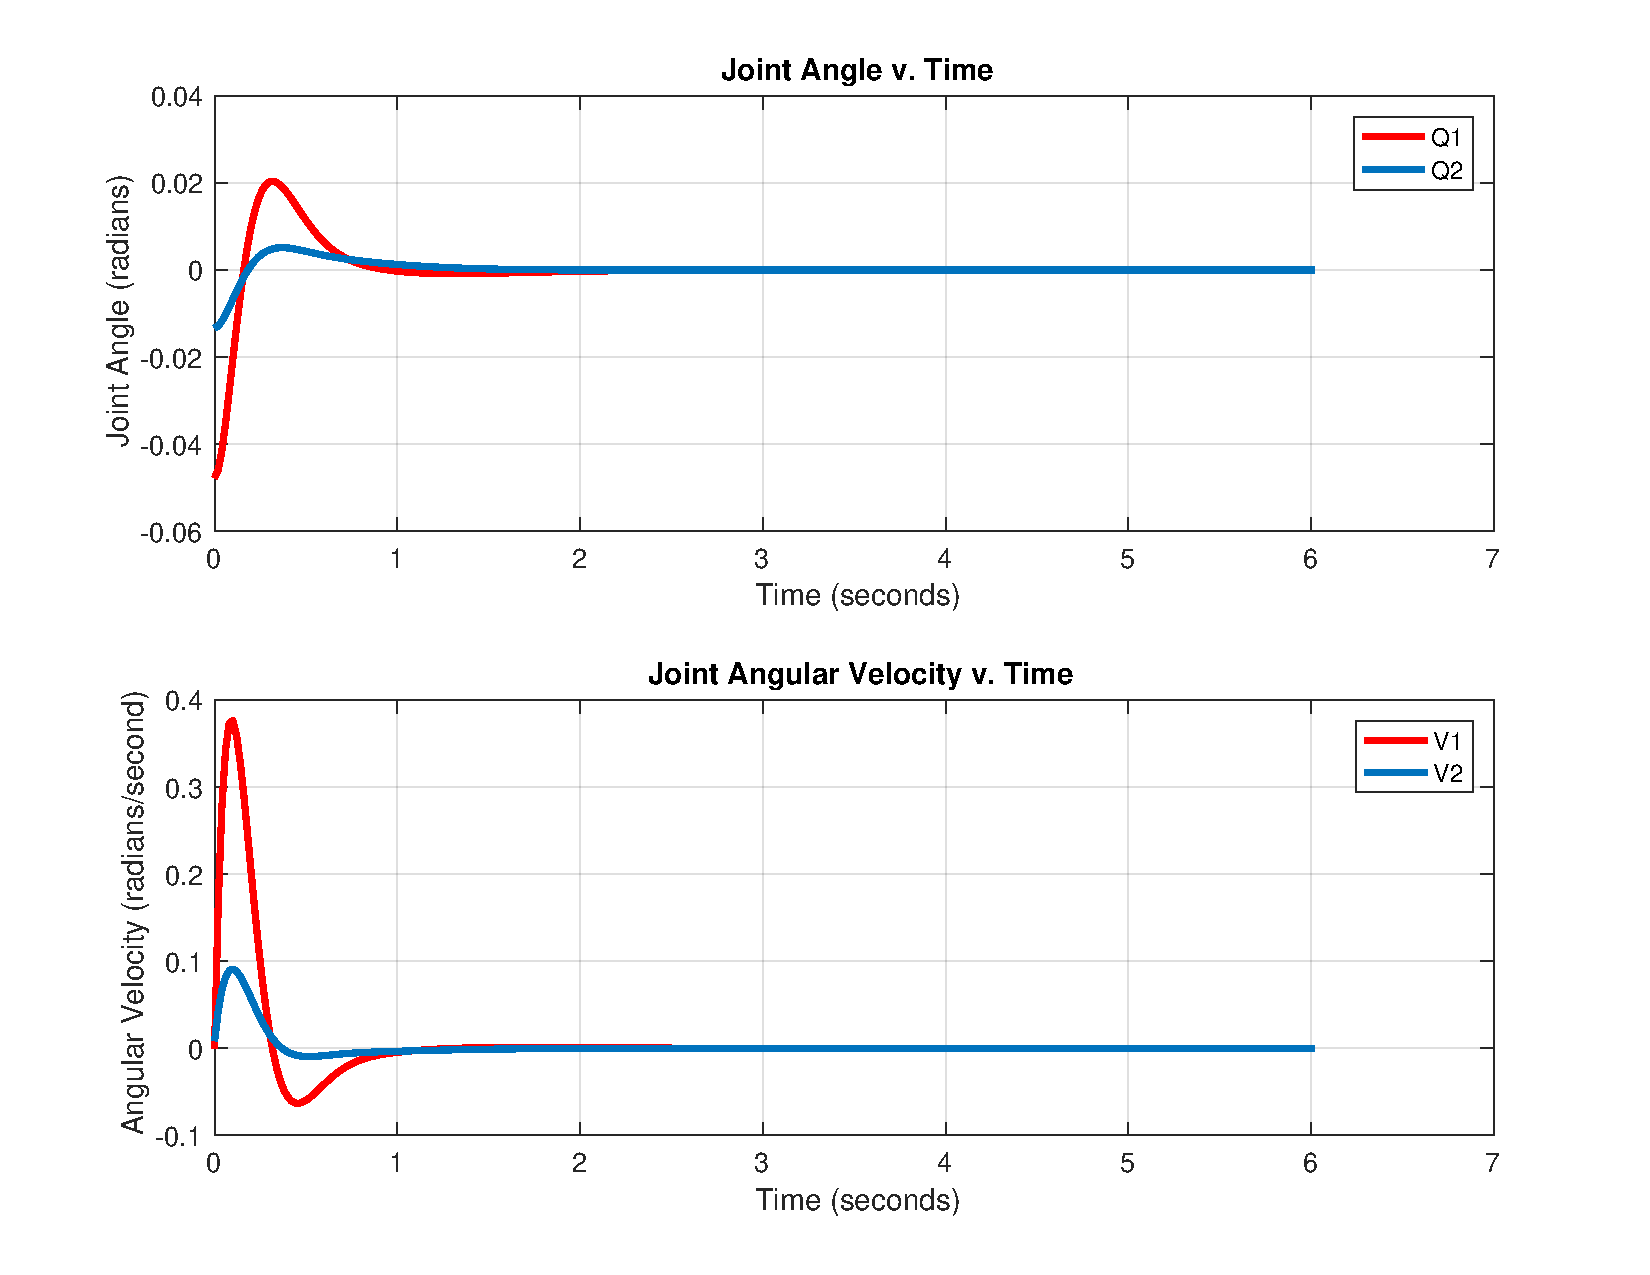
\includegraphics[width=0.5\textwidth]{statefeedrand.pdf}
\label{StateFeedback.c}}
\subfloat[Robotic arm with random initial conditions]{
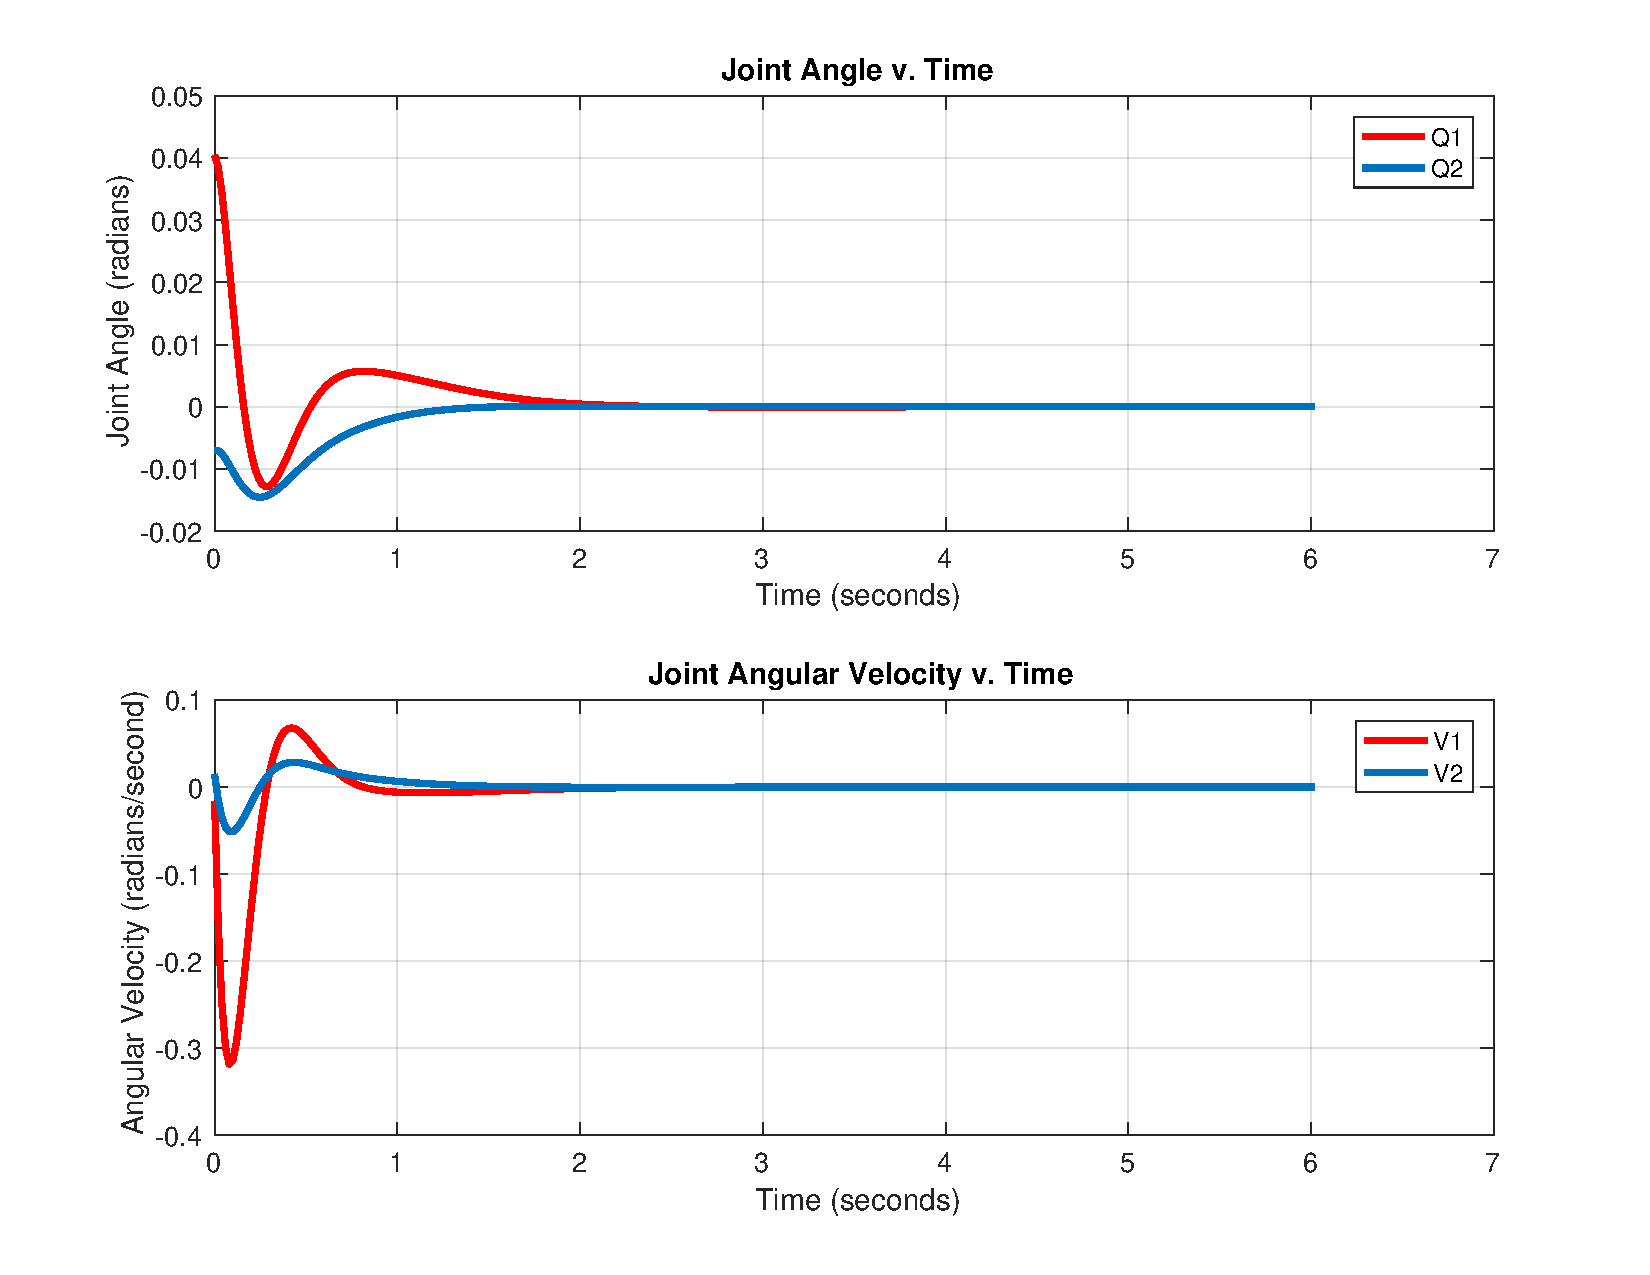
\includegraphics[width=0.5\textwidth]{statefeedrand1.pdf}
\label{StateFeedback.d}}
\caption{Joint angles and angular velocities of Robotic arm with a state feedback controller going to equilibrium.}
\label{StateFeedbackSet1}
\end{figure}
\clearpage
The matrices $Q$ and $R$ were used to calculate $K$. It can be seen in Figure \ref{diffQR} that if the penalties are changed, so will the convergence of the system. Figure \ref{diffQRa} shows the system when the penalty on the states is simply the identity matrix. Figure \ref{diffQRb} shows the system when the penalties acting on $q_{1}$ and $v_{2}$ are five while penalties on $q_{2}$, $v_{1}$ and $R$ are 50. Note the similarities between \ref{diffQRa} and \ref{diffQRb}. Figure \ref{diffQRc} shows the system when the penalties acting on $q_{1}$, $v_{2}$ and $R$ are five while penalties on $q_{2}$ and $v_{1}$ are 50. By changing $R$ to five, a clear change occurs in the sytem. The 'cost' that Q and R have on a system is a result of thier ratios. In \ref{diffQRb} the ratio of $Q$ to $R$ is the same as \ref{diffQRa} (in the places it counted). However, in \ref{diffQRc} the ratios are different which result in a stark difference in the system. Finally Figure \ref{diffQRd}  shows the system when induced to the original Q and R values introduced earlier in this section.
\\ \\
It should be noted that the plots in Figure \ref{diffQR} has the initial starting value of $\begin{bmatrix} q_{1} & q_{2} \end{bmatrix} = \begin{bmatrix} \pi & -\frac{6}{7} \pi \end{bmatrix}$. The initial value for $q_{2}$ was chosen as it is slightly off from a "natural" equilibrium point. Recall from the previous section how the natural equilibrium points were $\begin{bmatrix}q_{1} & q_{2}\end{bmatrix} = \begin{bmatrix}0 & 0\end{bmatrix}$ and $\begin{bmatrix}q_{1} & q_{2}\end{bmatrix} = \begin{bmatrix}\pi & -\pi \end{bmatrix}$. By defining $q_{2} $ as such, it can be assured that the system will be able to reach some equilibrium in time.
\begin{figure}[h!]
\centering
\subfloat[Q = \begin{bmatrix}
1 & 0 & 0 & 0 \\ 0 & 1 & 0 & 0 \\ 0 & 0 & 1 & 0 \\ 0 & 0 & 0 & 1
\end{bmatrix}
\qquad  
R = \begin{bmatrix}1\end{bmatrix}]{
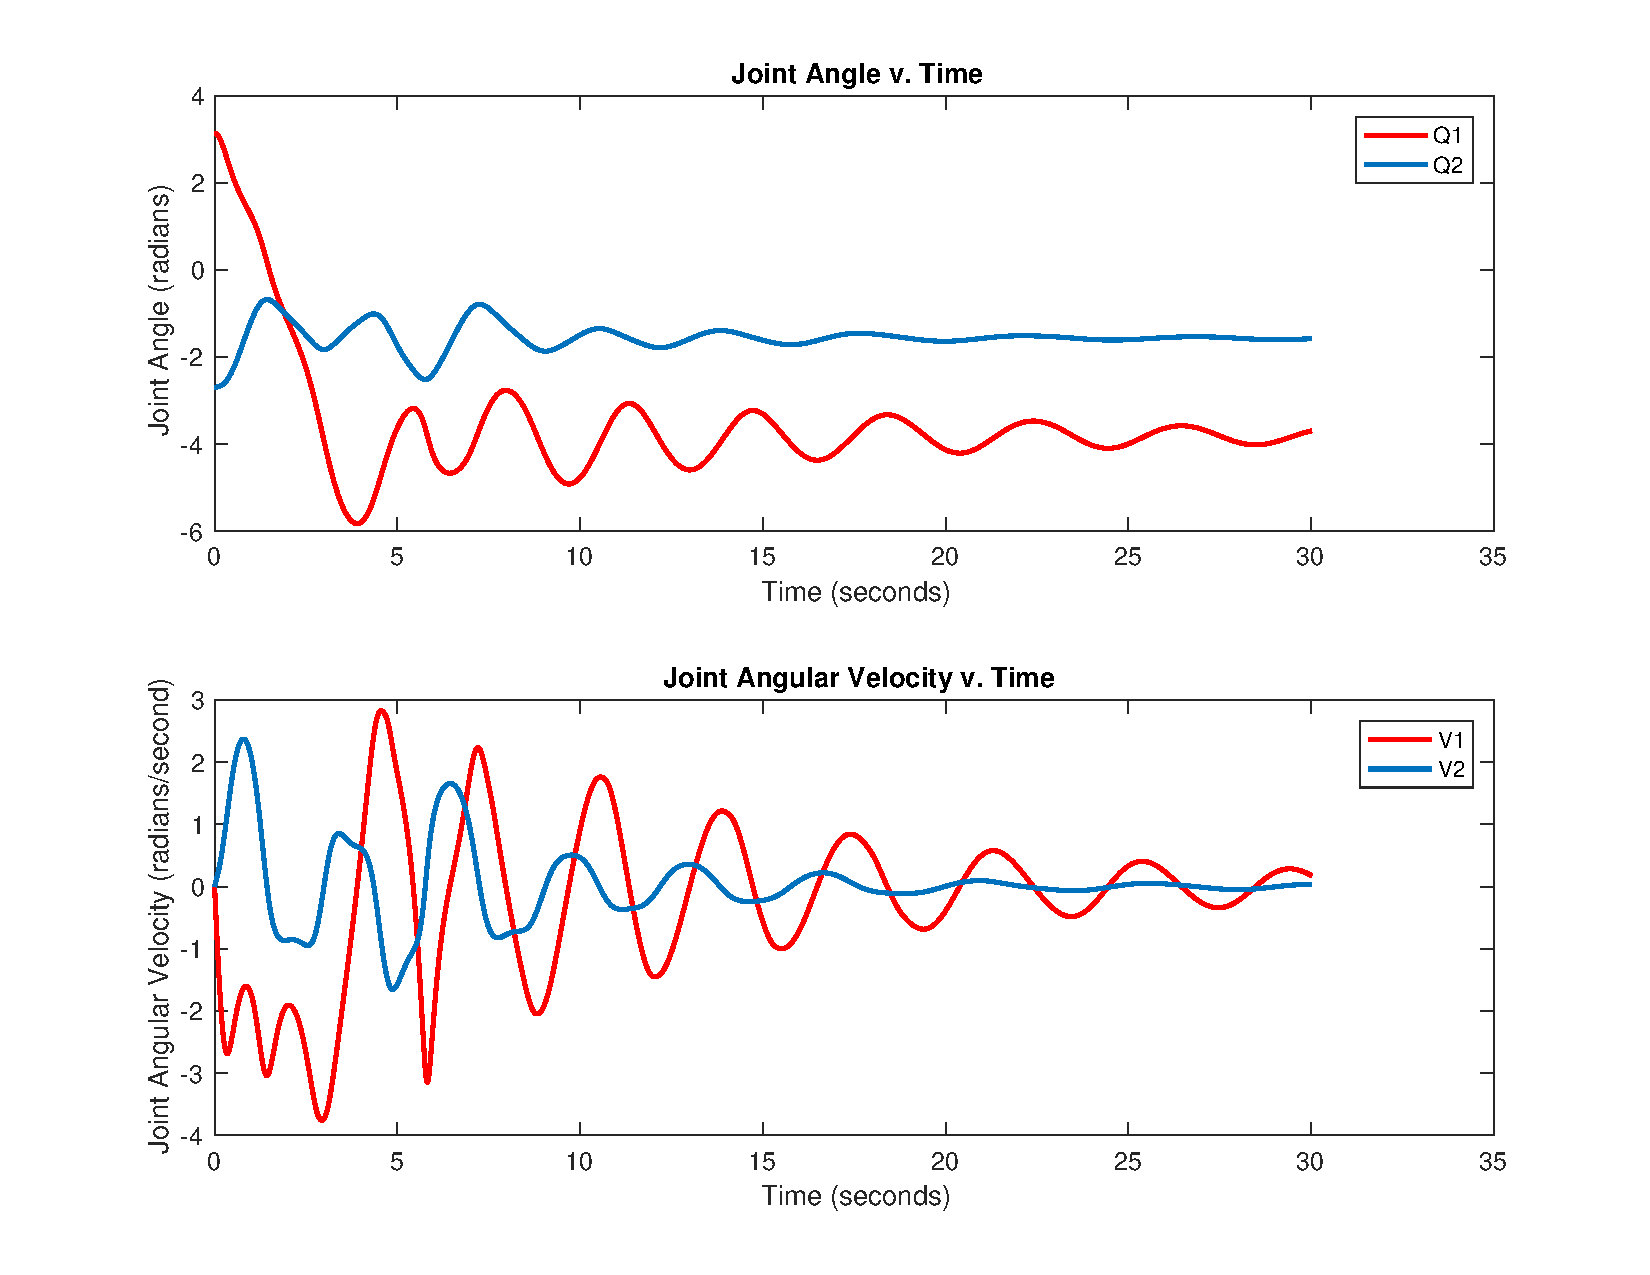
\includegraphics[width=0.5\textwidth]{q2.pdf}
\label{diffQRa}}
\subfloat[Q = \begin{bmatrix}
5& 0 & 0 & 0 \\ 0 & 50 & 0 & 0 \\ 0 & 0 & 50 & 0 \\ 0 & 0 & 0 & 5
\end{bmatrix}
\qquad  
R = \begin{bmatrix}50\end{bmatrix}]{
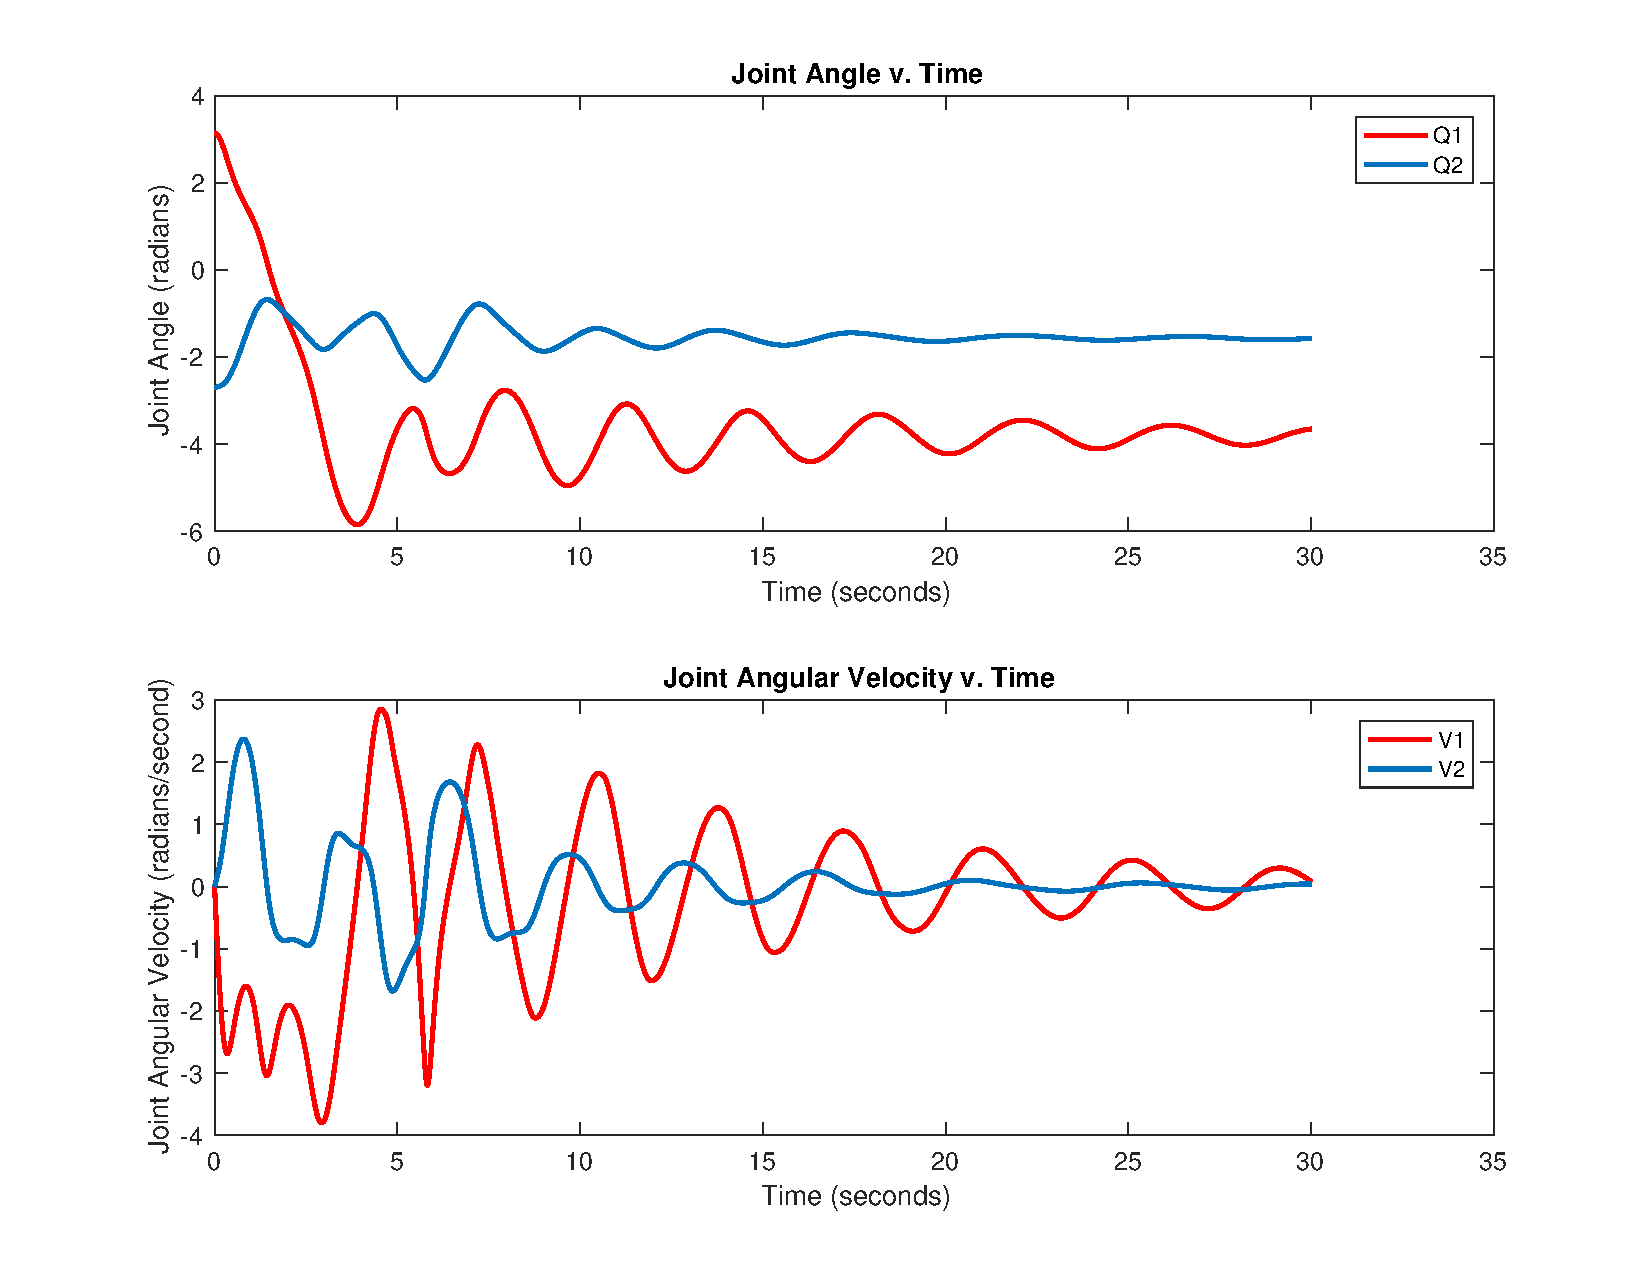
\includegraphics[width=0.5\textwidth]{q4.pdf}
\label{diffQRb}}
 \\
\subfloat[Q = \begin{bmatrix}
5& 0 & 0 & 0 \\ 0 & 50 & 0 & 0 \\ 0 & 0 & 50 & 0 \\ 0 & 0 & 0 & 5
\end{bmatrix}
\qquad  
R = \begin{bmatrix}5\end{bmatrix}]{
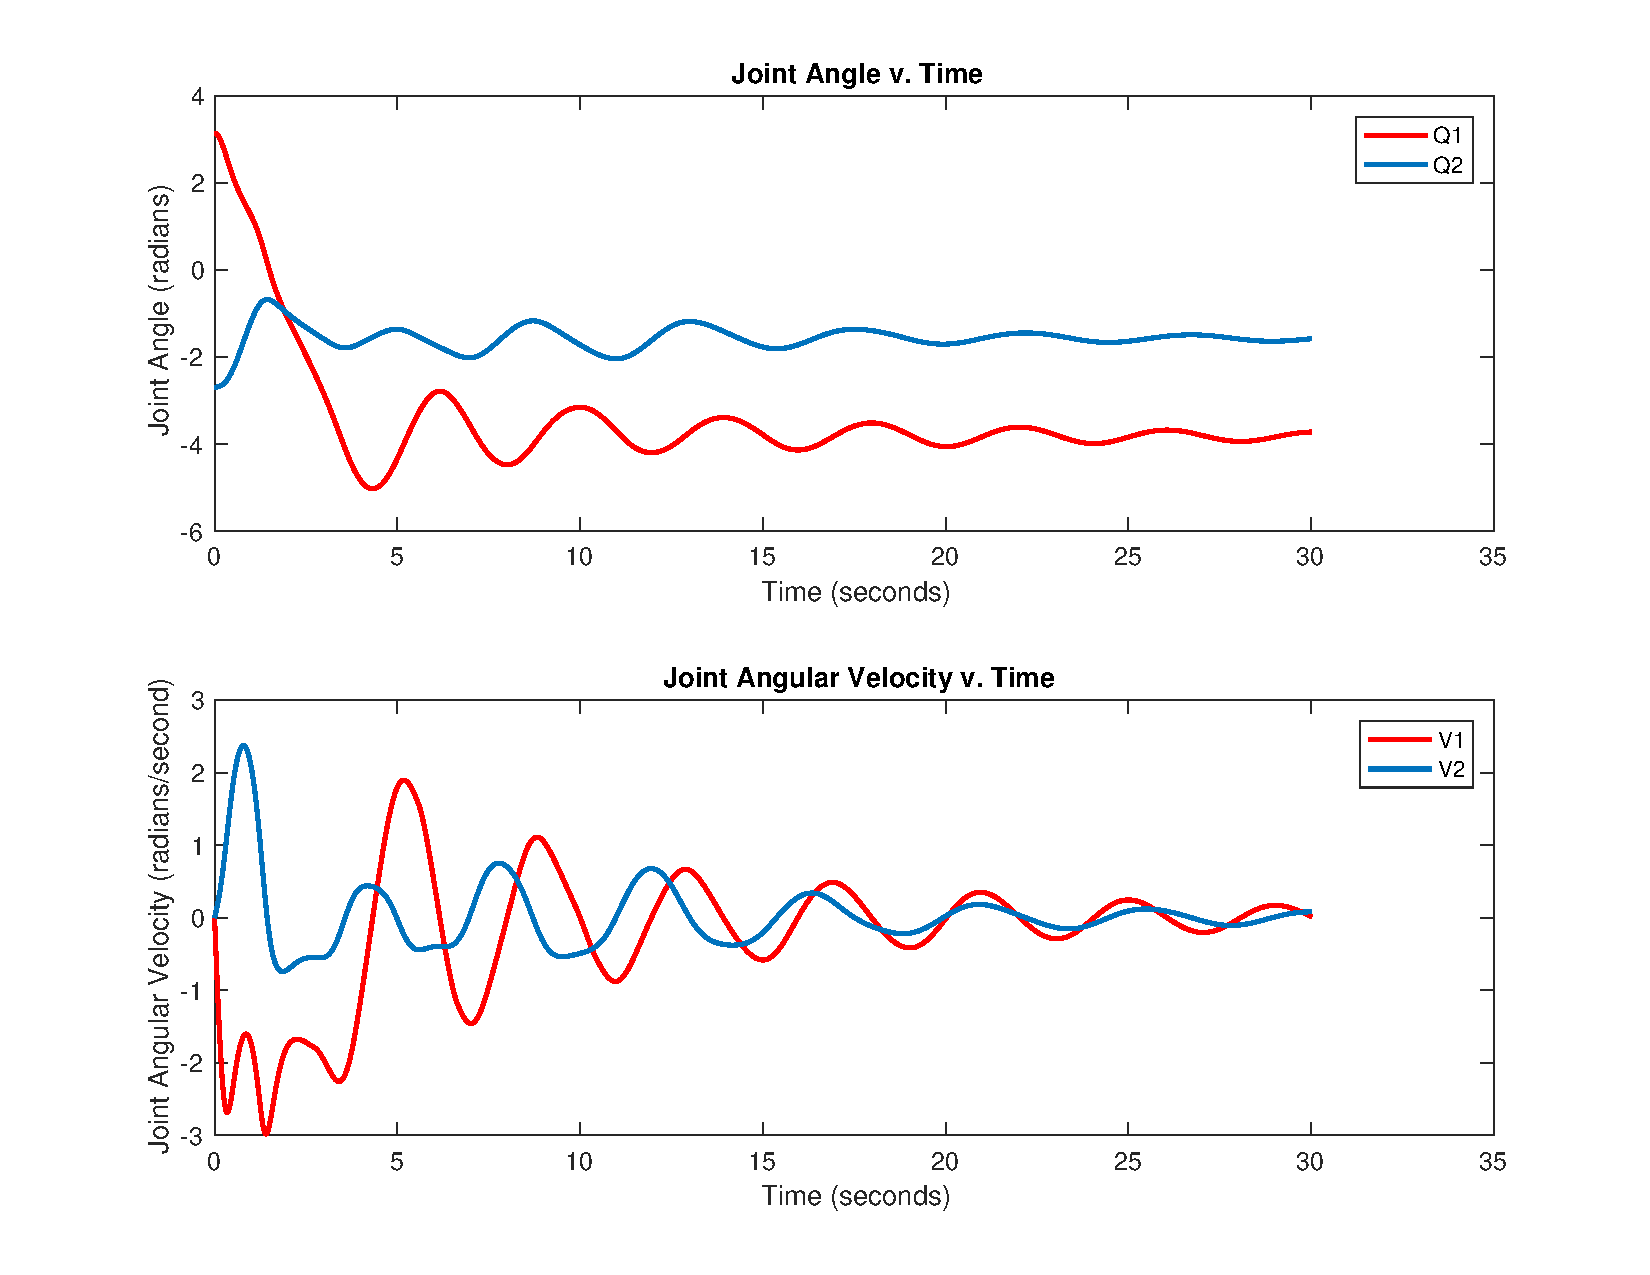
\includegraphics[width=0.5\textwidth]{q3.pdf}
\label{diffQRc}}
\subfloat[Q = \begin{bmatrix}
100 & 0 & 0 & 0 \\ 0 & 10000 & 0 & 0 \\ 0 & 0 & 1 & 0 \\ 0 & 0 & 0 & 1
\end{bmatrix}
\qquad  
R = \begin{bmatrix}1\end{bmatrix}]{
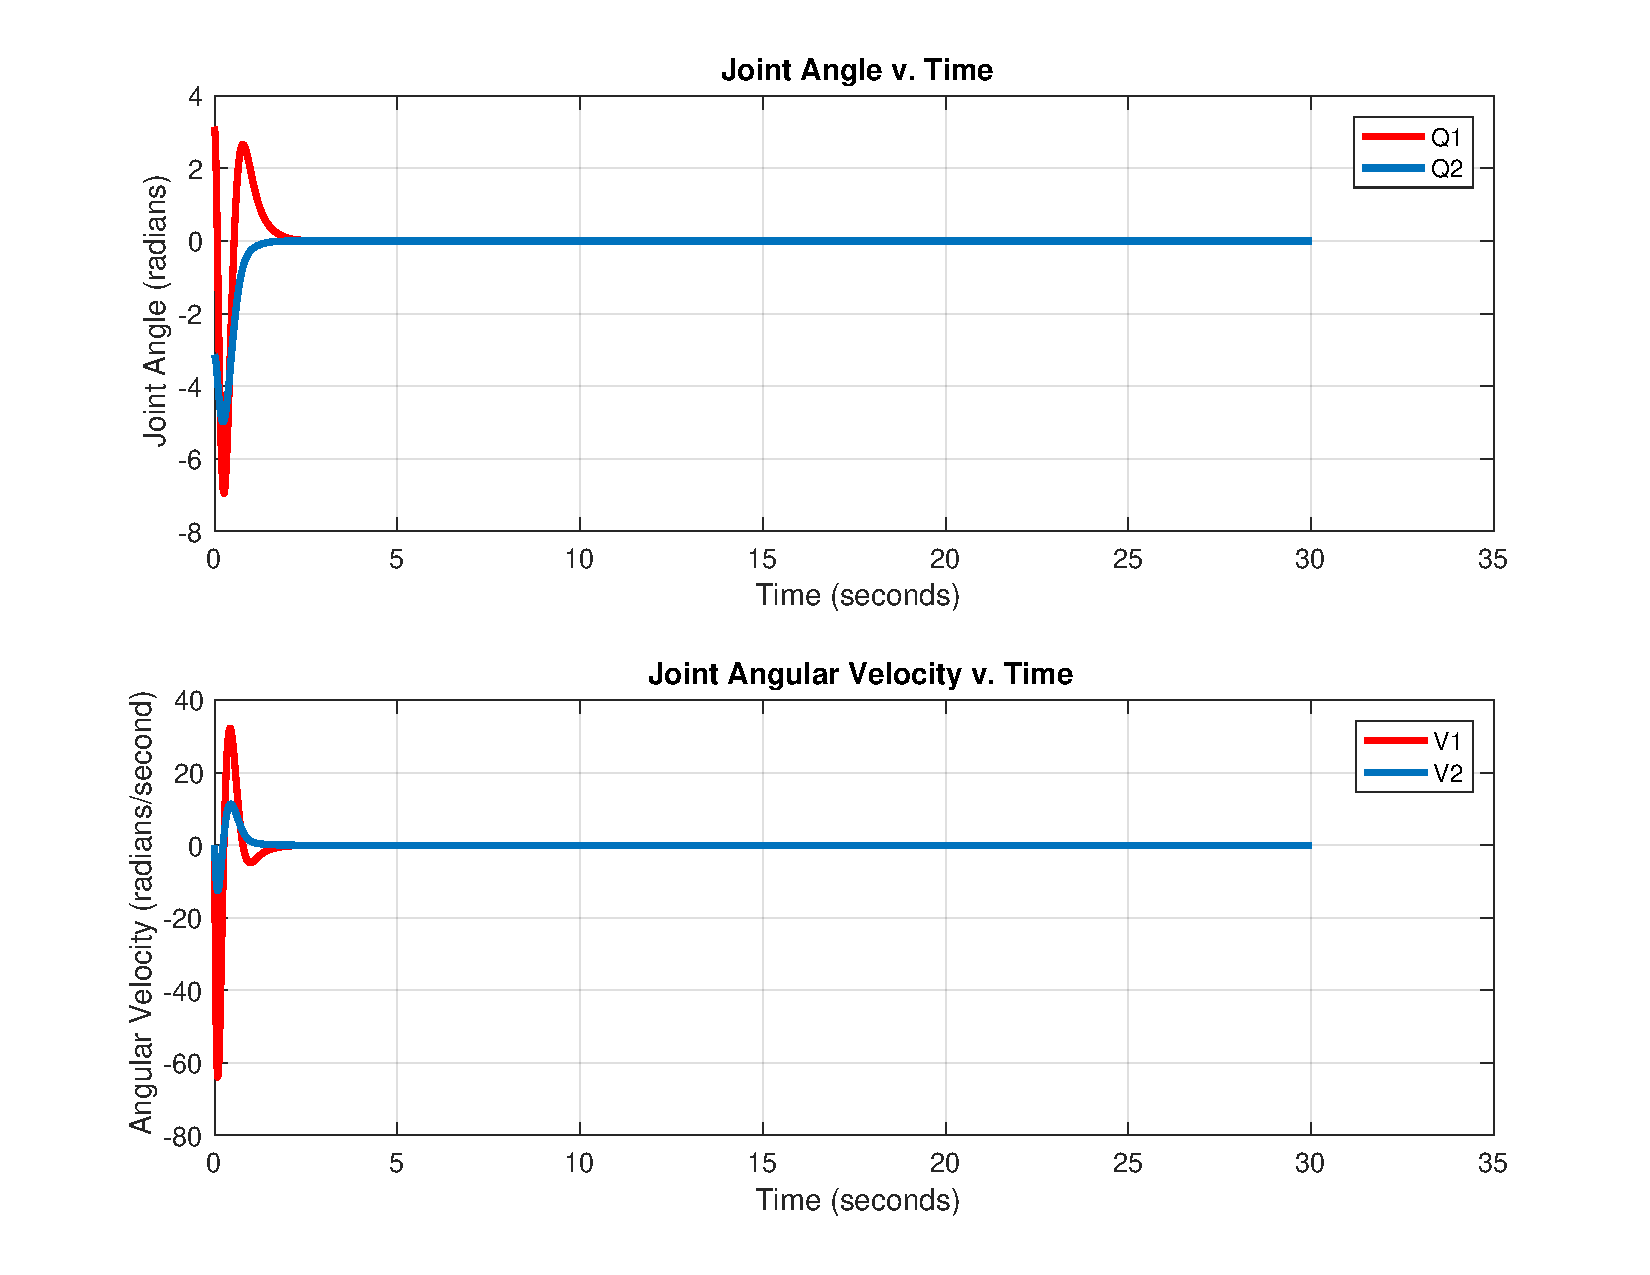
\includegraphics[width=0.5\textwidth]{q1.pdf}
\label{diffQRd}}
\caption{System undergoing different values of Q and R, thereby effecting K}
\label{diffQR}
\end{figure}
\clearpage 
\subsection{Stability}
At this time, both a open-looped zero-input system and a closed-loop state-feedback system have been tested. The stability of these systems can be determined by studying the eigenvalues of these systems. 
\\
For the case of a zero-input response, the following input to MATLAB is made for calculating the eigenvalues.
\begin{lstlisting}[frame=single]
[V,F]=eig(A) %Zero Input
\end{lstlisting}
For the case of state-feedback, the following input to MATLAB is made for calculating the eigenvalues.
\begin{lstlisting}[frame=single]
[V,F]=eig(A-B*K) %State Feedback
\end{lstlisting}
Where A, B and K are all predefined matrices for the state-space model. The term for which the eigenvector and eigenvalues is taken from is the term dependent on the state of the system as shown in Equation \ref{eqn10} as $A$ or $(A-BK)$
\begin{equation}
\label{eqn10}
\dot{x} = Ax
\qquad
\dot{x} = (A-BK)x
\end{equation}
After computing the MATLAB function, the matrices $V$ and $F$ are created. The matrices are structured such that the diagonal entries of $F$ are the eigenvalues of $A$ or $A-BK$.  These eigenvalues are denoted by $s_1$, $s_2$, $\hdots$, $s_n$, such that
\\
\begin{equation*}
F = 
\begin{bmatrix}
s_1 & 0 & \hdots & 0 \\
0 & s_2 & \hdots & 0 \\
\vdots & & \ddots & \vdots \\
0 & 0 & \hdots & s_n
\end{bmatrix}.
\end{equation*}
From this, it is found that the exponential of $F t$ produces the result
\begin{equation*}
e^{Ft}  =
\begin{bmatrix}
e^{s_1 t} & 0 & \hdots & 0 \\
0 & e^{s_2 t} & \hdots & 0 \\
\vdots & & \ddots & \vdots \\
0 & 0 & \hdots & e^{s_n t}
\end{bmatrix}.
\end{equation*}
The exponential establishes that the behavior of $x(t)$ is dependent on the entries in the matrix $e^{Ft}$. Two relations can be seen as a result
\begin{itemize}
  \item If $s_1$ is a positive real number, then $e^{s_1 t}$ grows exponentially as $t$ increases meaning the system is unstable.
  \item If $s_1$ is a negative real number, then $e^{s_1 t}$ decays exponentially to zero as $t$ increases meaning the system is stable.
\end{itemize}
With this information in mind, the stability for the zero-input open loop controller and the state-feedback closed-loop controller is verified. It is seen that the zero-input controller produces a positive eigenvalue verifying it is unstable. Opposing this, the state-feedback closed-loop controller has all negative real parts, verifying its stability.
\begin{equation*}
F_{ZeroInput}= 
\begin{bmatrix} 
2.7562 & 0 & 0 & 0
\\
0 & -4.2366 & 0 & 0
\\
0 & 0 & -1.0561 + 3.6854i & 0
\\
0 & 0 & 0 & -1.0561 - 3.6854i
\end{bmatrix}
\end{equation*}
\\
\begin{equation*} 
F_{StateFeedback}= 
\begin{bmatrix} 
-32.8790  & 0 & 0 & 0
\\
0 & -1.2210 + 1.8225i & 0 & 0
\\
0 & 0 & -1.2210 - 1.8225i & 0
\\
0 & 0 & 0 & -1.9273
\end{bmatrix}
\end{equation*}
\subsection{Reference Tracking}
The final controller to be added is reference tracking. With the implementation of reference tracking, the input is made to be linear to the reference point $r$. 
\\
\begin{equation}
\label{eqn11}
u = -K x + k_{ref} r
\end{equation}
Reference tracking introduces two new terms into the input equation, $k_{ref}$ and $r$. The value for $r$ represents the "reference." It chosen such that as $t \rightarrow \infty$ the value $y \rightarrow r$. For the purposes of achieving a robotic arm, this reference value is subject to change through the duration of the simulation. Despite this, the initial r value shall be set equal to equilibrium. The value for $k_{ref}$ is calculated such that the system reaches steady state. The definition of these two knew terms is expressed in Equation \ref{eqn13}. 
\begin{equation}
\label{eqn13}
r = \begin{bmatrix} 0 & 0 & 0 & 0\end{bmatrix}
\qquad
k_{ref} = \frac{1}{-C(A-BK)^{-1} B}
\end{equation}
\\ \\ 
It is important to note that the output of $k_{ref}$ is a 1x4 matrix whose entries are all zero except for the value which corresponds to $q_{2}$, the angle of the second joint. With this information, the two entries can be simplified to scalars 
\ref{eqn13}. 
\begin{equation}
\label{eqn13}
r = f(t)
\qquad
k_{ref} = \begin{bmatrix} 0 & -316.6672 & 0 & 0\end{bmatrix} = -316.6672
\end{equation}
acknowledging that $k_{ref}$ and $r$ only apply to $q_{2}$. Since the aforementioned goal for this system was to be able to track a sequence of reference points given by a function, $r$ is represented as a function of time. Any given function would be a possible reference value. However, given the constraints of the model and it's physical limitations, several factors should be kept in mind when choosing a formula for $r$ such that the system does not loose stability and to reduce the state error.
\begin{itemize}
	\item The function should start at the systems equilibrium at the time it is called. 
	\item The function should be continuouse
	\item If the system were to not be continuous and contain steps, the step intervals of the function should consider being less than one.
	\item The function should restrain from steep slopes.
\end{itemize}
These rules are not required in order for reference tracking to be successful however they greatly reduce the state error which is critical when considering the aforementioned goal. With these rules in mind and a certain personal vision for how the arm should behave, the following function for $f(t)$, the reference trajectory, was contrived.
\begin{equation*}
	f(t) = \frac{1}{5}\sin(0.1 t - 0.6)\cos(0.01 \pi t^{1.6} - 0.6)
\end{equation*}
With an understanding of waveforms, this function was created so have a reference path of a 'beating' wave with low amplitude and a large wavelength so to satisfy the rules above.
\\ \\
To implement reference tracking into the controller, a separate MATLAB script had to of been created. The function 'GenerateReferenceTrajectory'  completed this task and is shown in Figure \ref{figCodeRef}
\begin{figure}[h!]
\begin{lstlisting}
%Function GenerateReferenceTrajectory.m
function q2 = GenerateReferenceTrajectory(t)
    if t < 6
        %Reference Value from t=0 to t=6
        q2=0
    else
    	%Reference Value for t > 6
        q2 = SomeFunction f(t)
    end
end
\end{lstlisting}
\caption{Code to define and implement reference values for controller in MATLAB. 
\label{figCodeRef}}
\end{figure}
\\
The code from 'GenerateReferenceTrajectory' tells the system that for the first six seconds of the system, the reference point will be 0. There are several reasons why this was done. First, the goal is to have the robot arm stabilize to a predefined equilibrium value. This was stated to be zero. Finally, it allows the system to be at a recognized location once the reference trajectory comes into play. The function used was designed such that at $t=6$, $ref$ = f(t) = 0 and therefore would not be a shock to the system, potentially saving it from falling out of stability. It is clear in Figure \ref{refref} when reference tracking switches from being a constant value to the function $f(t)$. The next section will analyze the steady-state error between the reference trajectory and instantaneous $q_{2}$ values. In Figure \ref{refref2} the duration of the simulation was increased to 120 seconds. This better illustrates the desired shape of the function $f(t)$ and adds additional reasoning to the stability of this system. Had the time been extended even more, the 'beating' look that was desired would be even more apparent.
\begin{figure}[h!]
\centering
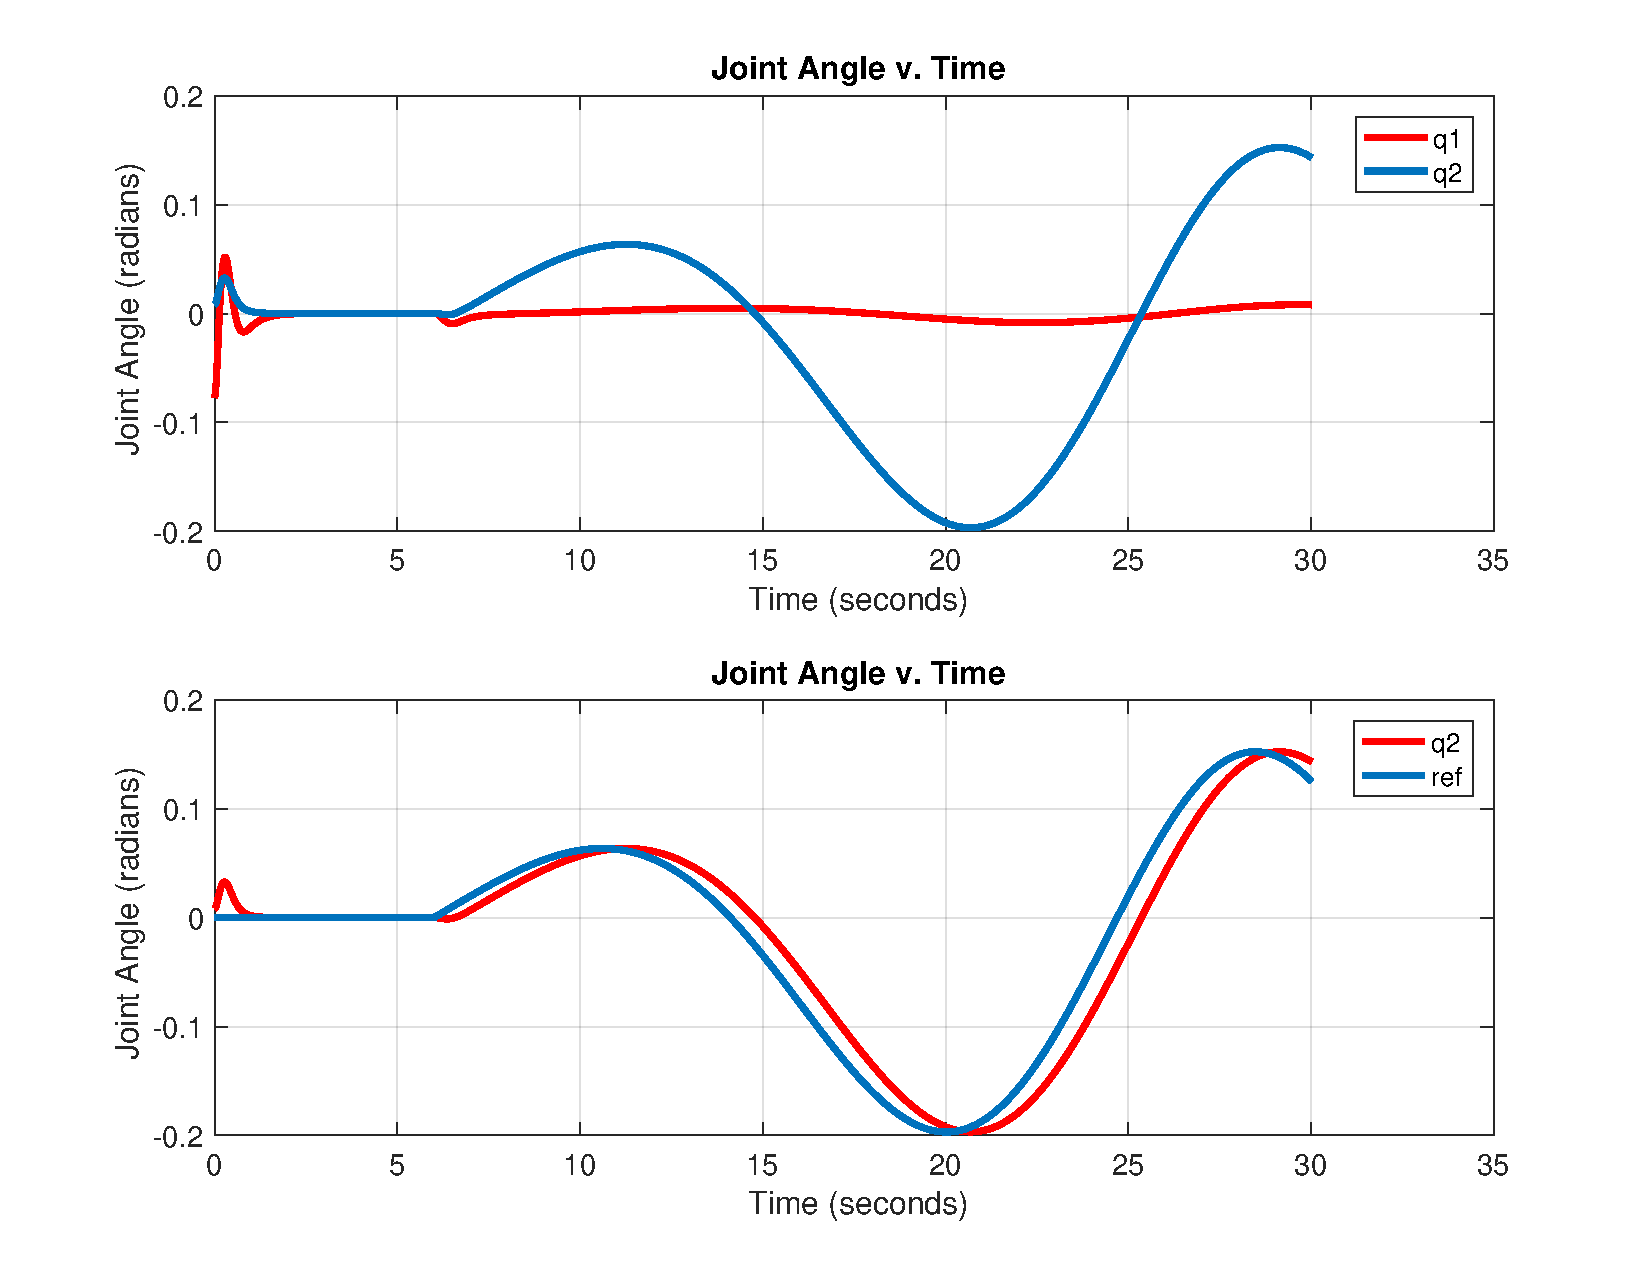
\includegraphics[width=1\textwidth]{RefTracking.pdf}
\caption{(top) Joint angles when reference tracking is applied. (bottom) Difference between reference and $q_{2}$ in time (30sec).}
\label{refref}
\end{figure}
\clearpage
\begin{figure}[h!]
\centering
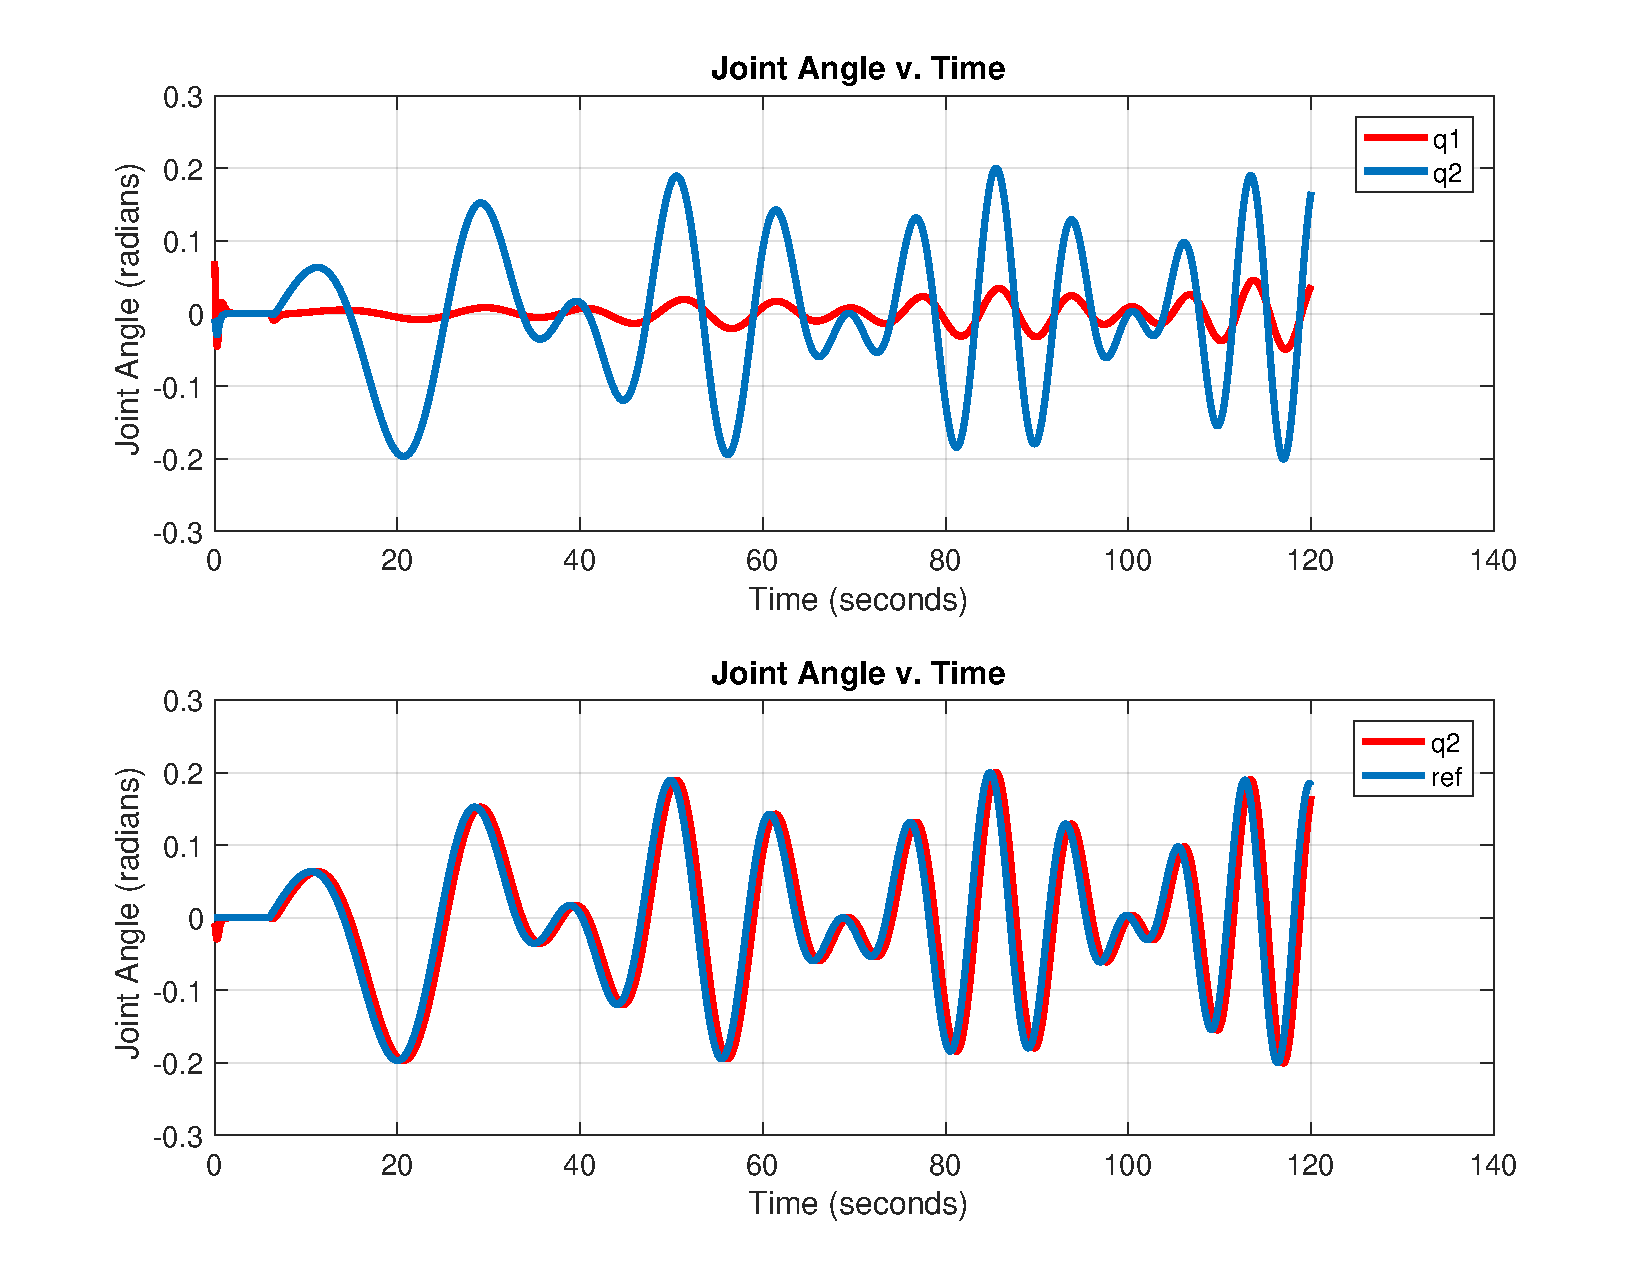
\includegraphics[width=1\textwidth]{RefTracking2.pdf}
\caption{(top) Joint angles when reference tracking is applied. (bottom) Difference between reference and $q_{2}$ in time (120sec).}
\label{refref2}
\end{figure}
\clearpage
\subsubsection{Steady State Error}
The controller section concludes with a discussion on steady-state error. Steady-state error is the difference between the steady-state output and the reference point. Since disturbance is simply the differnce between steady-state output and the reference point, it's units will be in radians. However, the goal is established in degrees so a simple conversion must be made. It can be observed in Figure \ref{error2a} that the steady-state error never exceeds a value greater than five.
\begin{figure}[h!]
\centering
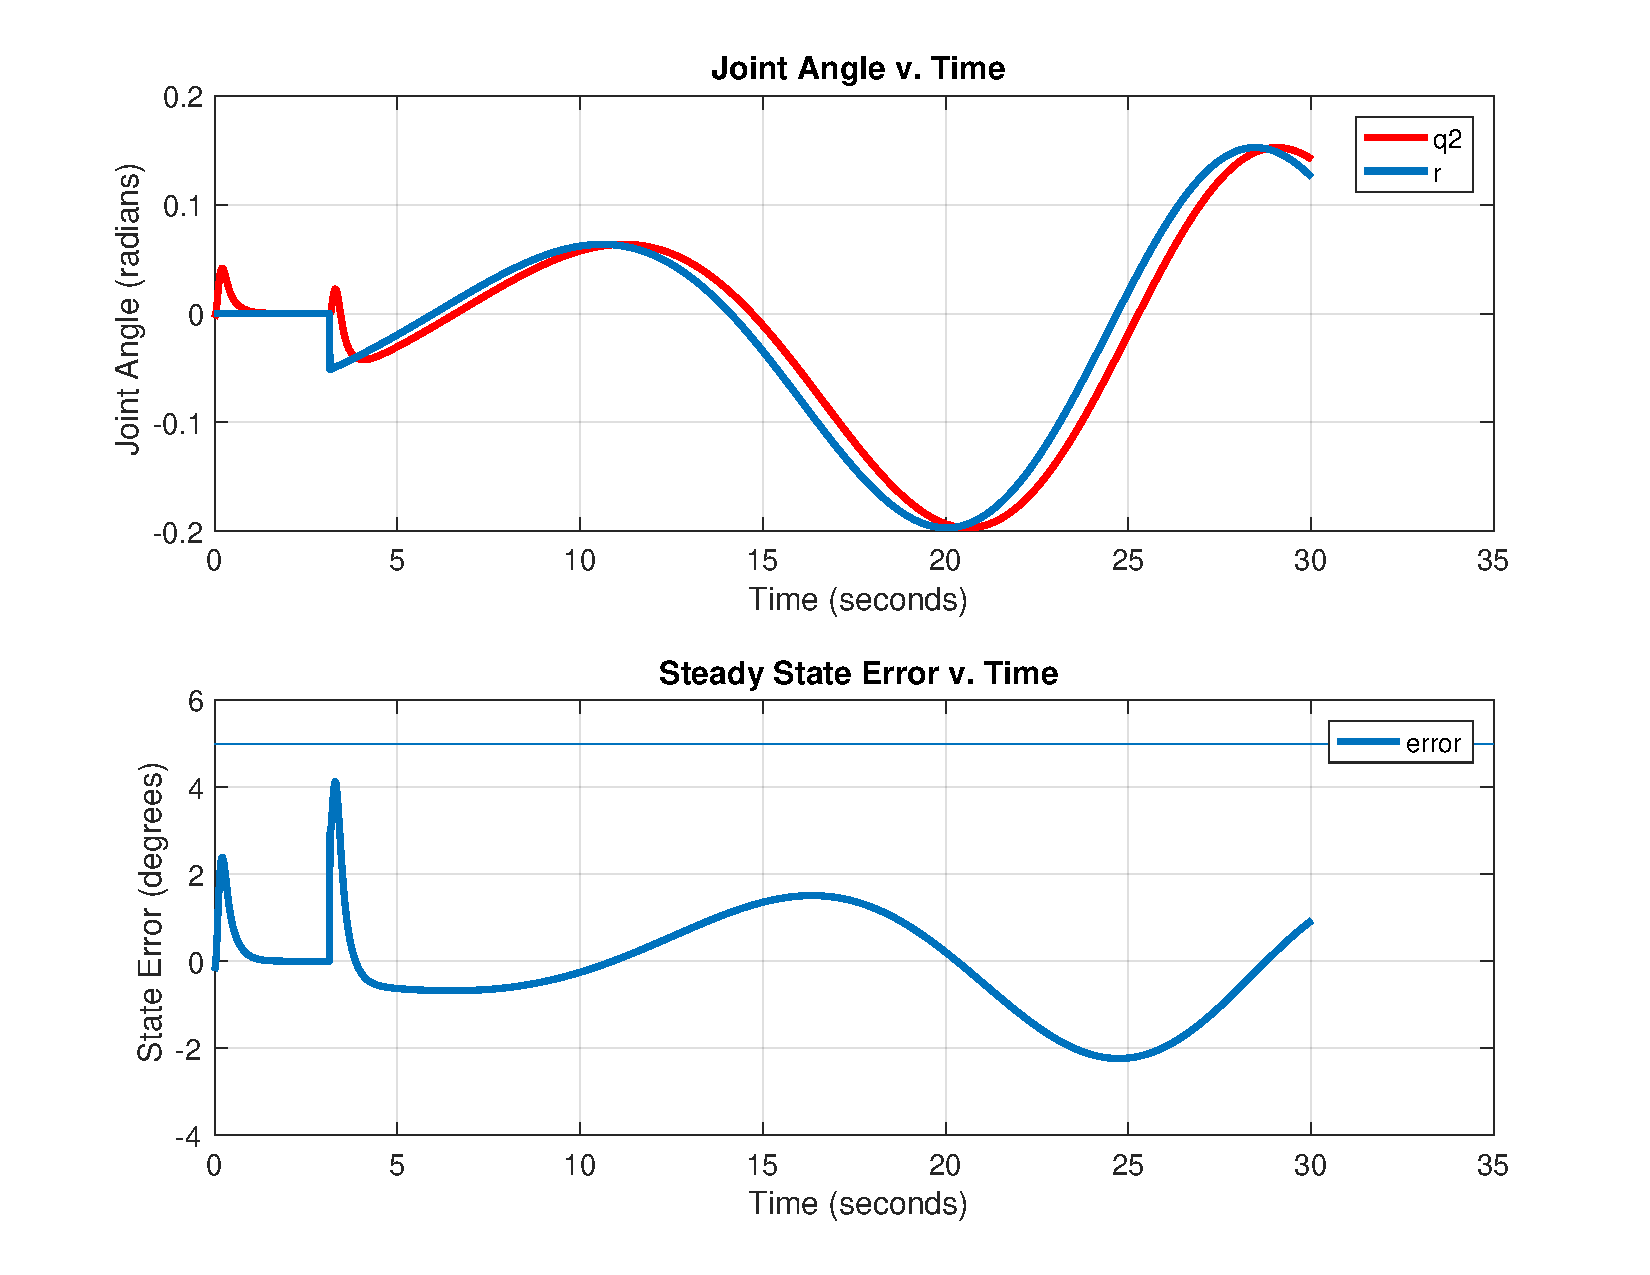
\includegraphics[width=1\textwidth]{StateErrorNormal.pdf}
\caption{Steady-State error without disturbance}
\label{error2a}
\end{figure}
\clearpage A factor that can be introduced into the system is disturbance. Disturbances are forces external to the system which are unknown and have an effect on the systems output. Disturbances can be accounted for by implementing integral action however, such steps were not taken for this system. By performing simulations with and without disturbance, an obvious increase in steady-state error depicted. It can be seen in Figure \ref{error2b} that the introduction of disturbance drastically influences the systems ability to reach the desired reference value, thereby increasing the steady-state error.
\begin{figure}[h!]
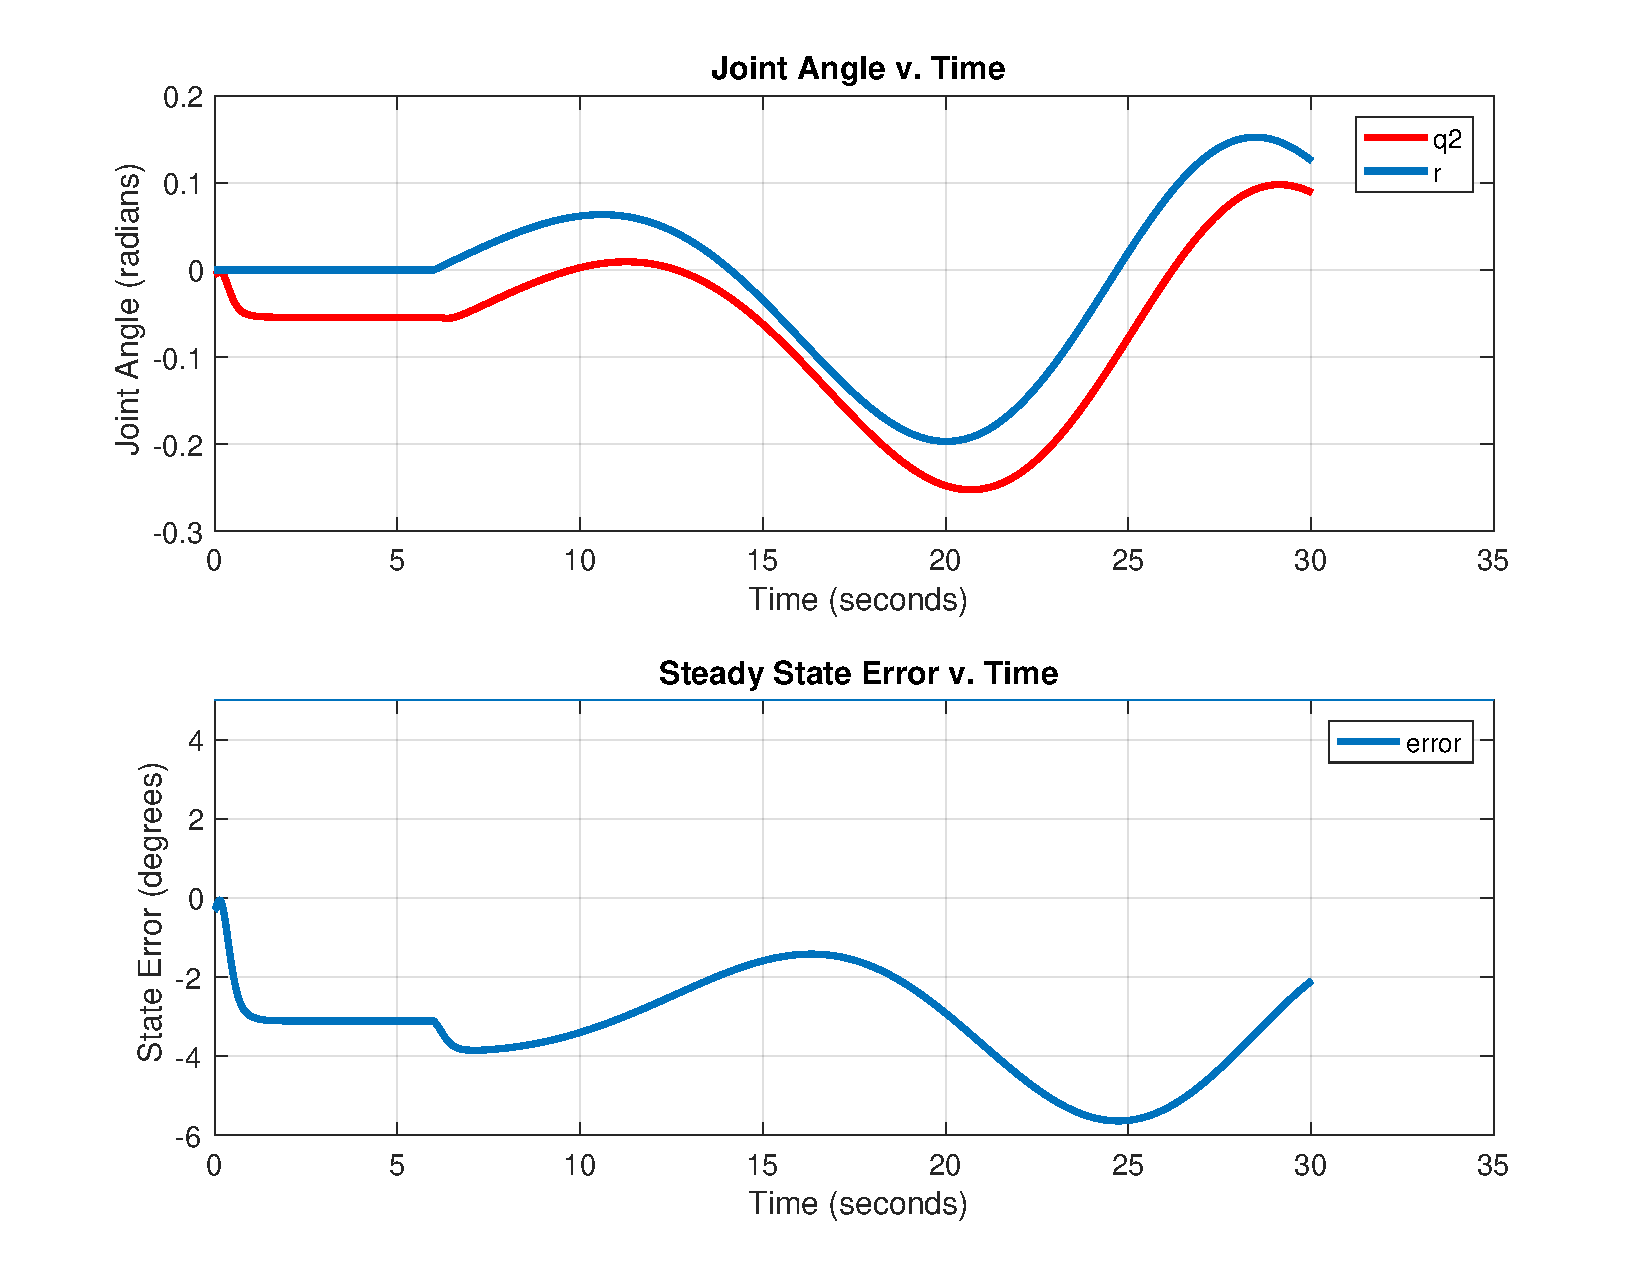
\includegraphics[width=1\textwidth]{StateErrorWithDisturbance.pdf}
\caption{Steady-State error with disturbance}
\label{error2b}
\end{figure}
\clearpage 
Prior to introducing disturbance, the maximum instance of state-error was less than $\pm5^{\circ}$. After introducing disturbance, the maximum instance of steady-state error is greater than $\pm5^{\circ}$. 

\section{Simulation Results}
In the first section of this report, a set of instructions was listed for verifying the requibments. To reiterate, these step are as follows
\begin{itemize}
	\item Devise a function to compute state error at every time interval.
	\item Plot a steady-state error to time curve. On this curve, include a reference line to mark when your steady-state error has surpassed the value stated by the requirment.
	\item Analyze the plot. If values exceed  $\pm5^{\circ}$, the single requirement has been ignored and the simulation has failed.
\end{itemize}
This procedure was conducted and the results are shown in Figure \ref{valid1}. By observing the plot, it is clear that the since the steady-space error does not surpass $\pm5^{\circ}$, the requirement is satisfied. 
\\
\begin{figure}[h!]
\centering
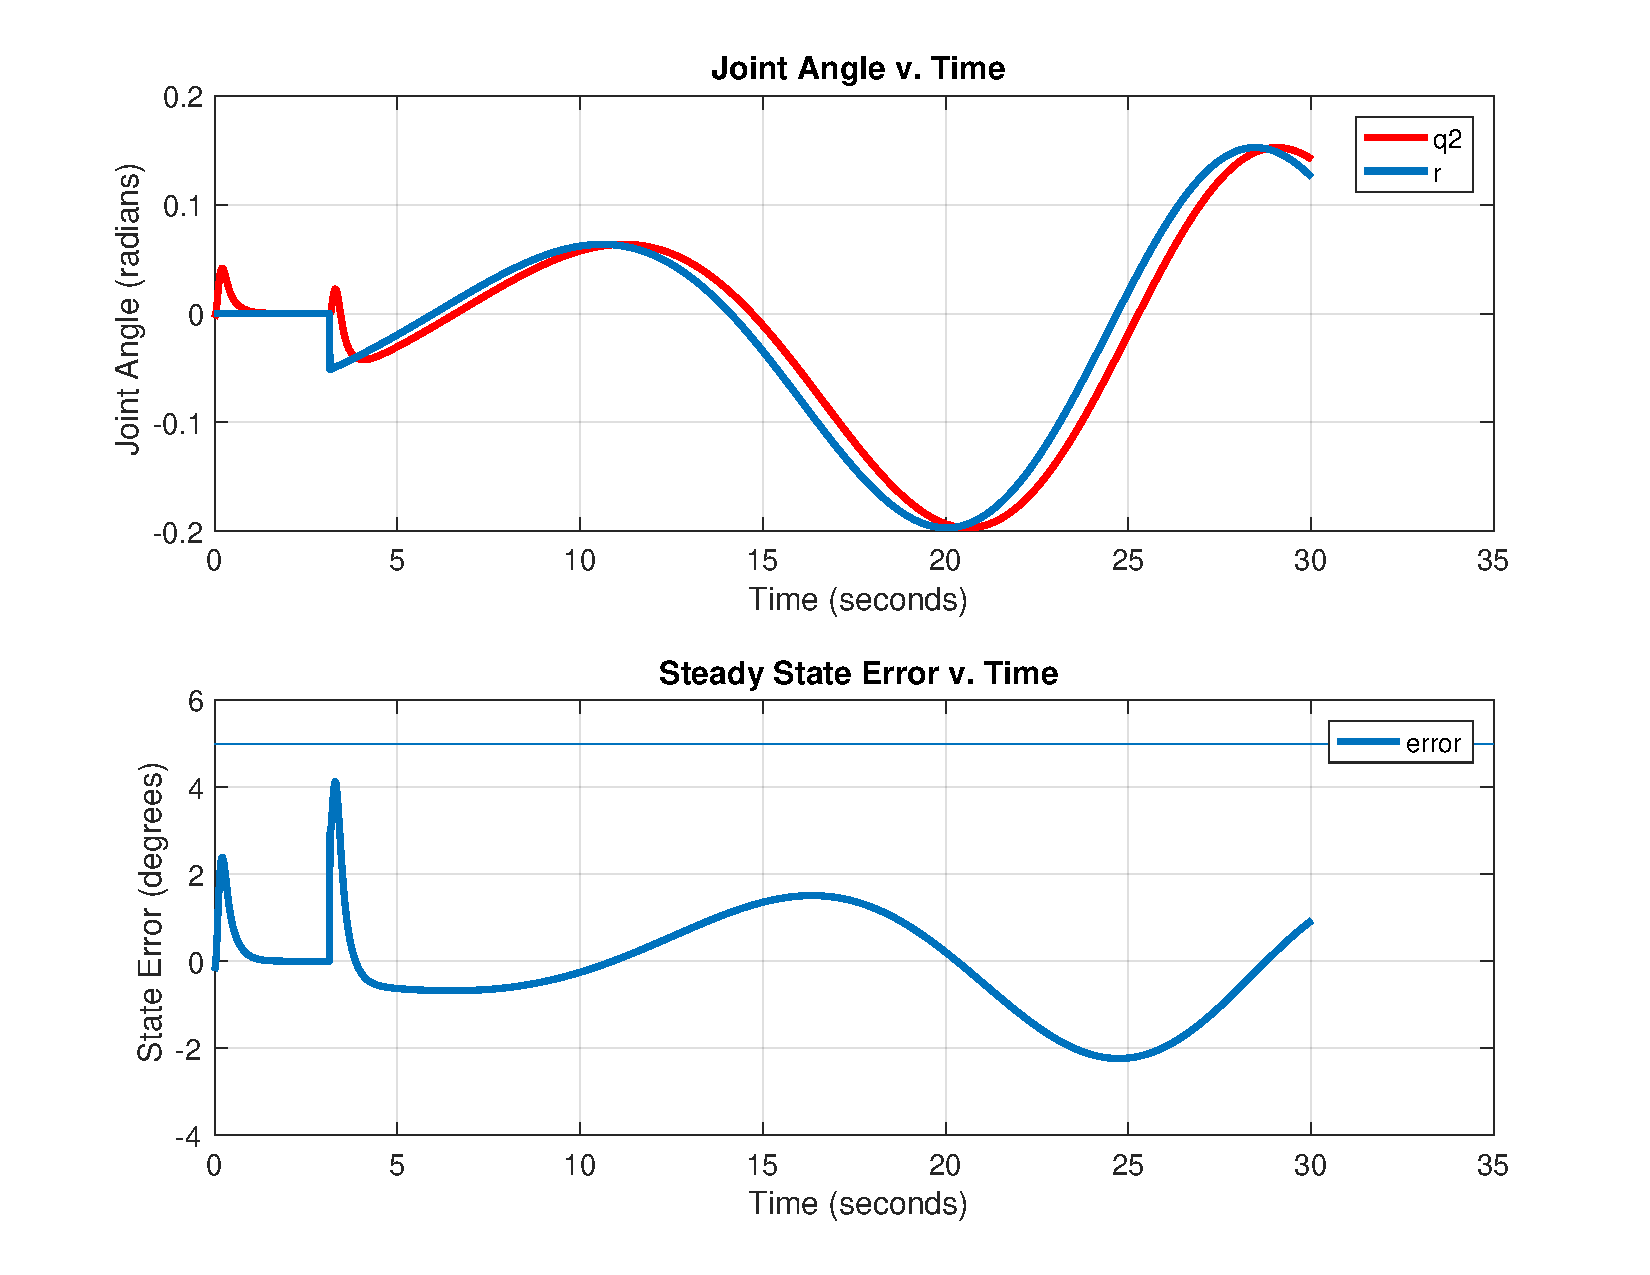
\includegraphics[width=1\textwidth]{StateErrorNormal.pdf}
\caption{Steady-State Error for 30 seconds. Requirement satisfied (pending)}
\label{valid1}
\end{figure}
\\ 
However, if the timeframe of the simulation is extended as shown in Figure \ref{valid2}, the requirement ends up not being satisfied. This is clearly a result of reference equation chosen since it is expected to get oscillate more rapidly as time advances. It was explained earlier how the structure of the waveform can have effects on the state-error of the function and how the speed of oscillations prevent the system from reaching the reference value fast enough.
\\
\begin{figure}[h!]
\centering
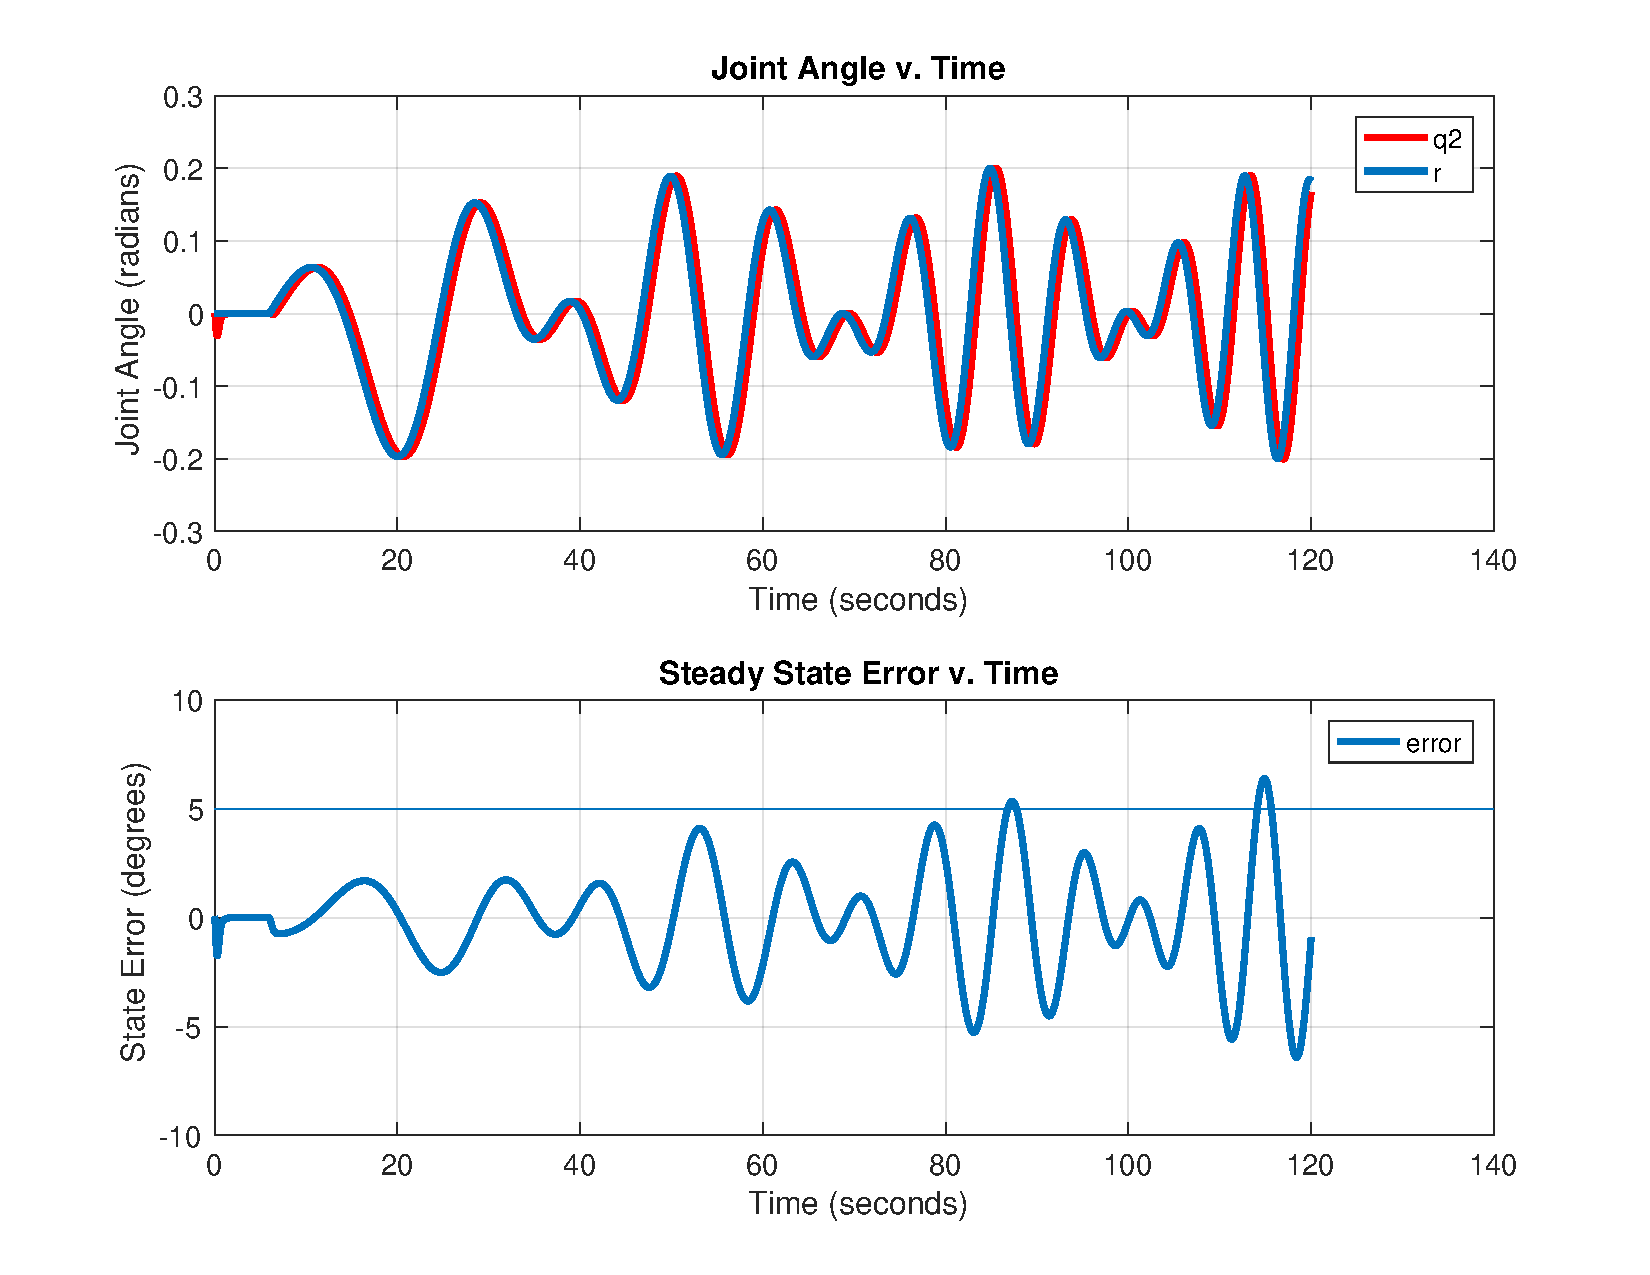
\includegraphics[width=1\textwidth]{StateError120.pdf}
\caption{Steady-State Error for 120 seconds. Requirement unsatisfied}
\label{valid2}
\end{figure}
\\
An alternative equation using a more simple reference trajectory is shown in Figure \ref{valid3}. It is apparent by looking at the plot that the steady-state error never exceeds $\pm5^{\circ}$ thus satisfying the established requirement and proving that the function chosen to be the reference trajectory has an effect on steady-state error.
\begin{figure}[h!]
\centering
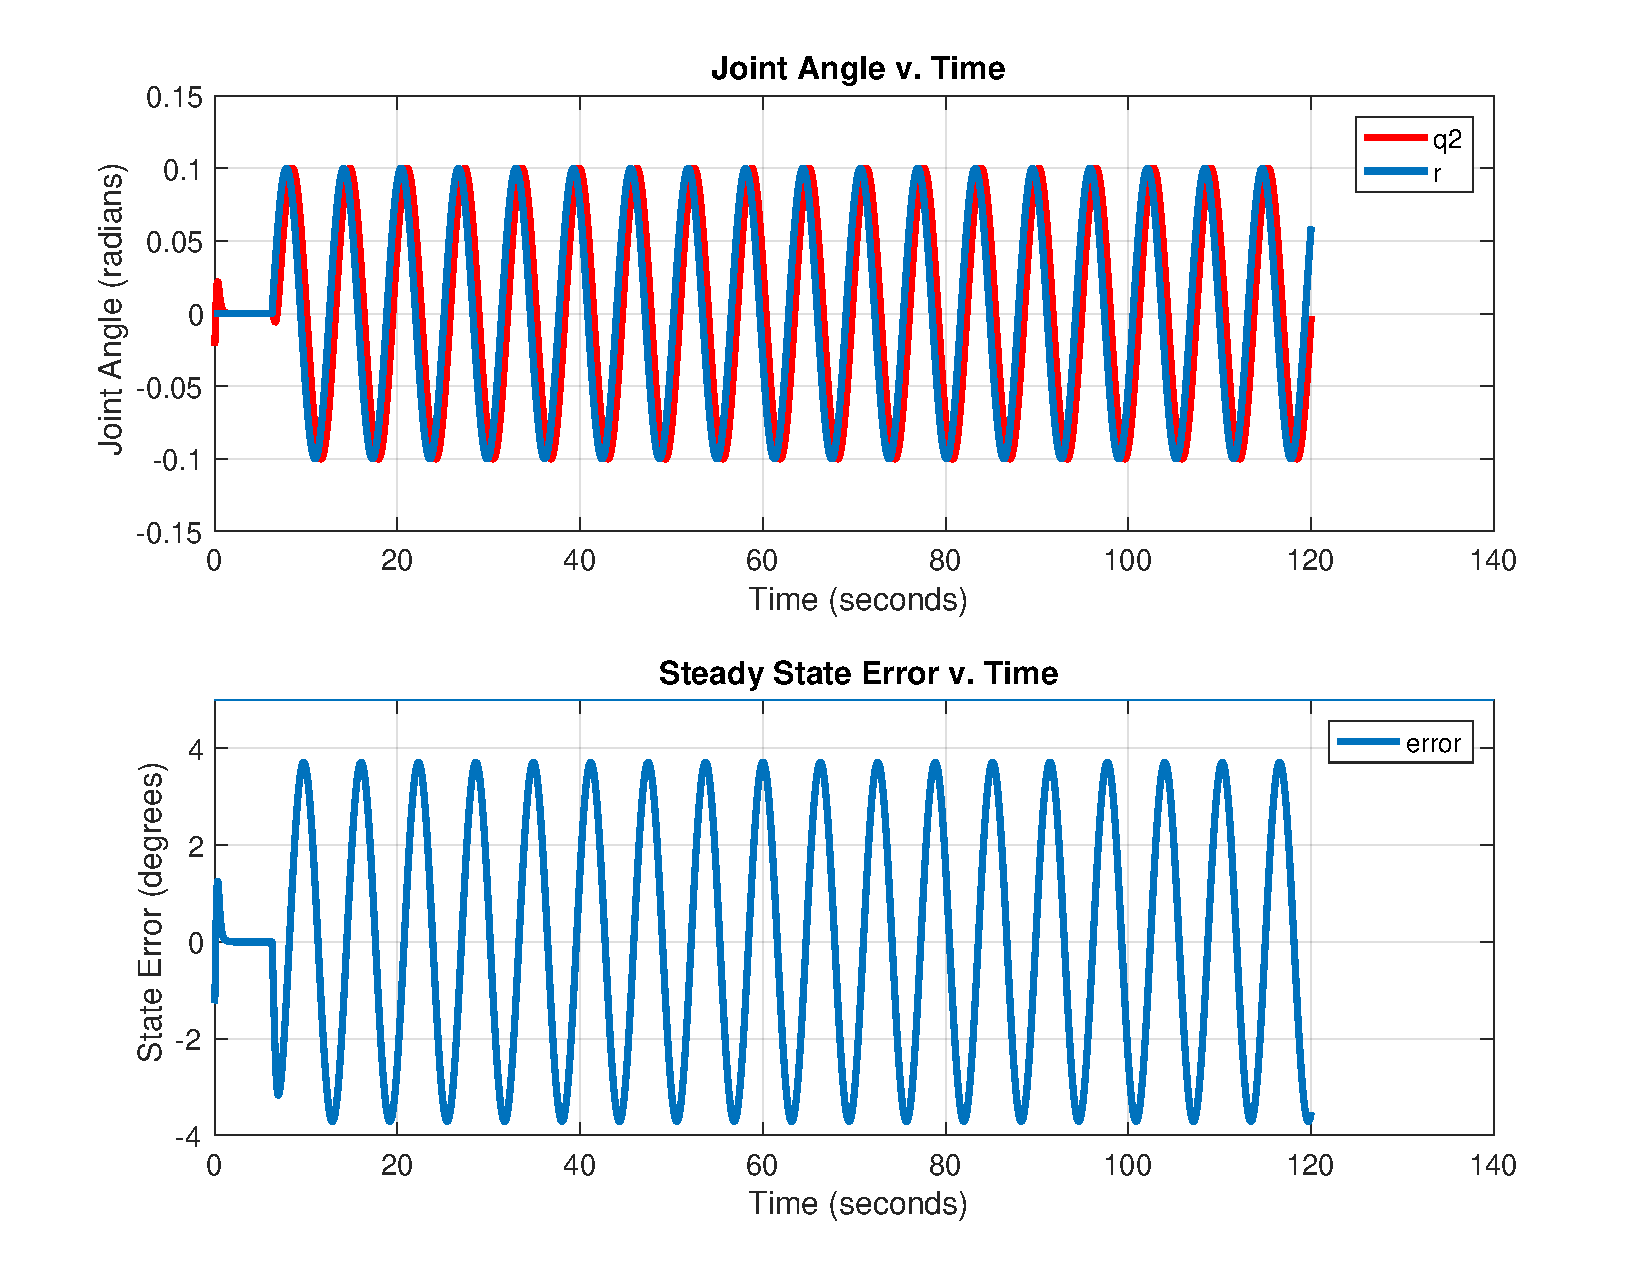
\includegraphics[width=1\textwidth]{StateErrorAltEqn.pdf}
\caption{Steady-state error with a reference trajectory of $r(t)=0.1\sin(t)$. Requirement satisfied (always)}
\label{valid3}
\end{figure}
\\
\clearpage

\section{Conclusion}
In this report, a gravity-assisted under actuated robotic arm was tasked to track a given reference trajectory within a  $\pm5^{\circ}$ margin of error. A simulation was conducted to determine if this goal was achievable. The requirements set for the model were that the second joint angle shall remain within $\pm5^{\circ}$ of its instantaneous reference through-out the duration of the simulation. This requirement was then verified by computing the error at every instance of time and through repeated simulation. The error was then plotted and any points exceeding $\pm5^{\circ}$ were noted and signified the requirement was not satisfied. If no point exceeded  $\pm5^{\circ}$ then the requirement had been satisfied. 
\\ \\
The results conclude that this goal is feasible. The robotic arm can remain within a $\pm5^{\circ}$ margin of error given certain conditions for the reference trajectory. Achieving this goal required the system to first be linearized. This was made simple through Matlab. Following that, the open-loop linear system was tested and confirmed for controllability using the controllability matrix and rank comparison. The open-loop linear system was used to compute the eigenvalues to determine if it were stable. After the open-loop linear system proved to have been unstable, a closed-loop state feedback controller was implemented. This system used a linear quadratic regulator to determine an optimal K value which in turn produced an efficient way of reaching equilibrium. Once proven to have been stable, reference tracking was implemented which allowed for the continuous tracking of a reference trajectory which is user controlled. Finally, a function for steady-state error was used to verify the results and confirm that the goal is obtainable since the requirements were satisfied (with some exceptions).

% Display list of references in IEEE Transactions format.
\bibliographystyle{IEEEtran}
\bibliographystyle{IEEEtran}
\bibliography{references}



% End of document (everything after this is ignored)
\end{document}